This chapter presents technical background information required to understand this thesis
and discusses related work from the perspective of industry and academia.
\Cref{s:process-security-model} presents technical background on historical models for
process-level confinement, with a particular emphasis on Multics, Unix, and Unix
derivatives.  \Cref{s:security-extensions} focuses on subsequent extensions to the Unix
security model and covers related work in the confinement space. \Cref{s:virtualization}
examines process-level virtualization technologies in Unix-like operating systems.
\Cref{s:containers-bg} discusses the differences between hypervisor- and container-based
virtualization, container security, and presents related work in the container security
space. Finally, \Cref{s:ebpf-bg} presents a detailed history of \glsentryshort{ebpf},
describes its architectural components and features, and discusses use cases in security
and beyond.

\section{Classic Unix Process Security Model}%
\label{s:process-security-model}

This section reviews foundational concepts in \gls{os} (particularly Unix-like \gls{os}s
and Linux) security. In particular, we discuss the \textit{reference monitor concept},
\textit{virtual memory and user processes}, and \textit{discretionary access control} and
how these concepts interact to form the backbone of process-level security in Unix.  The
goal of this section is to help the reader build a mental model of how operating systems
isolate and protect processes and system resources at the most fundamental level. Readers
familiar with these \gls{os} security concepts can skip this section in favour of
\Cref{s:security-extensions} which examines more advanced security mechanisms and
discusses related work.

\subsection{The Reference Monitor}%
\label{ss:refmon}

The \textit{reference monitor concept}, first introduced in the landmark 1972 Anderson
Report~\cite{anderson1972_report}, was among the earliest complete descriptions of a full
access control mechanism and remains influential in operating system design to date. The
reference monitor is an abstract model for a secure reference validation mechanism built
into the operating system. The model partitions the system into \textit{subjects} (users,
processes, etc.) and \textit{objects} (system resources).  Subjects request access to
objects and the reference monitor checks this access against a known list of allowed
accesses, parameterized by the subject, object, and requested access. The software
implementation of a reference monitor is known as the \textit{security kernel.}
\Cref{fig:refmon} depicts the reference monitor concept as it was first presented by
Anderson~\cite{anderson1972_report}.

\begin{figure}[htbp]
  \centering
  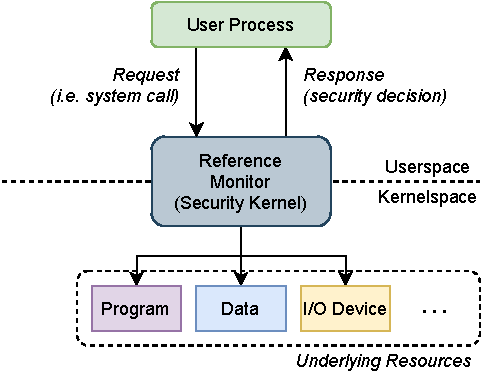
\includegraphics[width=0.6\linewidth]{figs/background/refmon.pdf}
  \caption[The reference monitor concept]{
    The reference monitor concept as outlined in the Anderson Report. Redrawn and adapted
    from Anderson~\cite{anderson1972_report}. User processes make requests (e.g.\ via
    system calls to the operating system). The \gls{os} kernel invokes the reference
    monitor, which is implemented in software as a security kernel. The reference monitor
    queries its security policy taking the subject, object, and other parameters as input.
    As output, it returns a security decision (i.e.\ whether the requested access should be
    \textit{allowed} or \textit{denied}).
  }%
  \label{fig:refmon}
\end{figure}

While the majority of modern operating systems do not include a security kernel as
described by Anderson, the reference monitor architecture has informed the design of
modern access control mechanisms and models the reference validation process that occurs
when the kernel is servicing userspace requests (i.e.\ system
calls)~\cite{van_oorschot2020_tools_jewels}. In order for such a design to be considered
valid, Anderson enumerates three key properties: (i) Tamper Resistance; (ii) Complete
Mediation; and (iii) Verifiability. These properties facilitate reasoning about the
security of modern access control mechanisms, even if they do not strictly adhere to the
reference monitor model.

\paragraph*{Tamper-Resistance}

In order for the reference monitor to be considered \textit{tamper-resistant}, an unauthorized
party must not be able to alter the reference monitor's code or modify any data
(e.g.\ memory, persistent storage) that the reference monitor relies on to enforce correct
reference validation~\cite{anderson1972_report}. This property follows from the fact that
unauthorized tampering with the reference monitor totally invalidates any security
guarantees.

\paragraph*{Complete Mediation}

The property of \textit{complete mediation} means that the reference monitor should be
invoked on all security sensitive events. It should be impossible for an attacker to
bypass the reference monitor in any way. Any software that is not subject to reference
validation should be considered a part of the reference
monitor~\cite{anderson1972_report}.

\paragraph*{Verifiability}

\textit{Verifiability} refers to the ability to reason about or prove the correctness of
the reference monitor (i.e. that the first two properties hold). Formal verification methods
are the best way of achieving verifiability, although this may not necessarily be practical
for highly complex systems. For this reason, it is recommended to design the reference monitor
in such a way that verifiability is maximized~\cite{anderson1972_report}.

\subsection{Virtual Memory and Memory Protection}%
\label{ss:virtual-memory}

Virtual memory~\cite{denning1970_virtual} is a mechanism for mapping \textit{virtual}
memory addresses to \textit{physical} machine addresses. First introduced in the 1950s,
the original goal of virtual memory was to make it easier for programmers to manipulate
memory without worrying about the underlying details of storage
configuration~\cite{denning1970_virtual}. With the advent of multi-processing systems,
virtual memory took on a new role\,---\,separation of memory resources between distinct
user processes. This separation is a fundamental notion for secure multi-processing; two
user processes should not be able to interfere with each other's memory, and a user
process should not be able to interfere with the \gls{os} kernel, resident in ring
0 memory.

By partitioning memory into virtual address spaces, virtual memory forms the most
fundamental isolation barrier between user processes. To accomplish this goal, a hardware
mechanism, the \gls{mmu}, translates virtual addresses to physical addresses using
a \textit{page table} maintained by the operating system in main memory. To accelerate the
translation of memory addresses, modern processors cache this mapping in a specialized
cache area called the \gls{tlb}.  In Unix, each user process gets its own virtual address
space by default, maintained in a per-process page table. Where necessary, this isolation
may be voluntarily broken using memory sharing mechanisms provided by the \gls{os} kernel
(e.g.\ multi-threading or shared memory mappings). The kernel also gets its own address
space which maps the entirety of physical memory.

While virtual memory can help isolate user processes from each other and user process from
the kernel, additional protection mechanisms are required to strengthen this isolation. To
this end, the \gls{cpu} \gls{isa} generally defines memory protection bits that can be applied
to physical pages and enforced in the \gls{mmu}. For instance, individual pages can be
marked as readable, writable, and/or executable depending on how the memory is to be used.
How these protections are used is generally up to the operating system; for instance,
modern operating systems often enforce a policy where pages marked writable and not
allowed to be marked executable and vice versa (this is often referred to as W$\oplus$X).
This helps to prevent the most baroque code execution attacks. Another important
protection mechanism employed by the operating system is \gls{aslr}, which slightly
randomizes virtual address space mappings, making them unpredictable and thus harder for
attackers to exploit consistently. A similar mechanism, \gls{kaslr}, protects the kernel.
The \texttt{grsecruity} patch suite~\cite{grsecruity} offers additional memory protection for the
Linux kernel, hardening the boundary between userspace and kernelspace and applying
additional mitigations to prevent return-oriented programming attacks.

Additional protections are afforded by \textit{memory protection rings}, a concept first
introduced by Multics~\cite{vyssotsky1965_multics, corbato1965_multics} in the mid-1960s.
In the original design, 64 protection rings were defined in hardware, numbered from 0--63.
A task running in a higher-numbered protection ring would be unable to access any memory
marked with a lower-numbered protection ring, effectively isolating sensitive code and
data from unprivileged tasks. Modern \glspl{cpu} carry forward this notion of protection rings,
although a typical modern processor only defines \textit{four} protection rings rather
than 64. Modern \gls{os}s, including Linux, generally only use \textit{two} of these
rings, ring 0 and ring 3 for kernelspace and userspace respectively. \Cref{fig:rings}
depicts this design. Lee \etal~\cite{lee2018_lotr} have proposed using the remaining two
rings for finer-grained isolation on x86.

\begin{figure}[htbp]
  \centering
  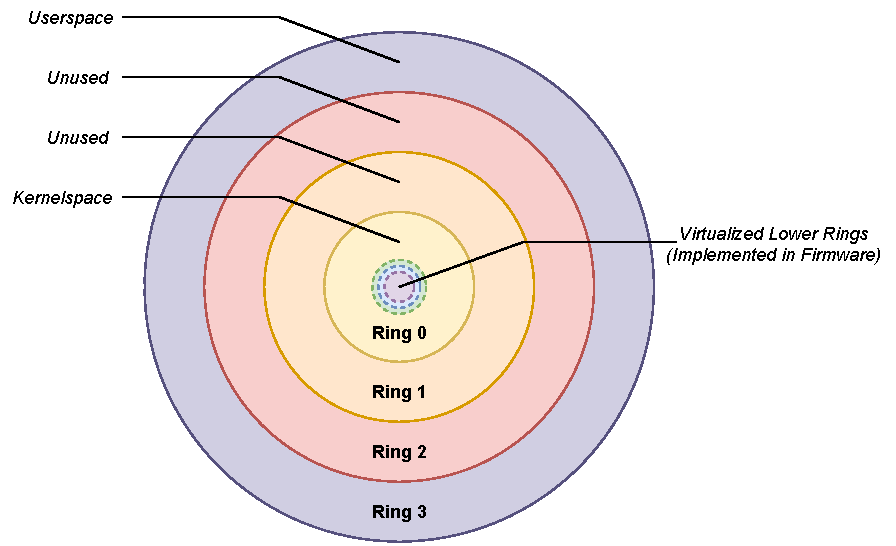
\includegraphics[width=0.8\linewidth]{figs/background/rings.pdf}
  \caption[Protection rings on modern \glsentryshortpl{cpu}]{
    A visualization of protection rings on modern \glsentryshortpl{cpu}. Ring 3 contains
    \textit{userspace}, the address space of ordinary applications that run in user mode.
    Ring 0 contains \textit{kernselspace}, the kernel's address space. Code running in
    ring 0 is said to run in \textit{supervisor mode}. Rings 1--2 are generally unused by
    \glsentryfull{cots} operating systems.  Modern \glsentryshortpl{cpu} often implement \enquote{lower}
    rings (-1, -2, etc.) by virtualizing ring 0 in firmware. These are typically reserved
    for the hypervisor and other hardware-backed features like Intel's System Management
    Mode~\cite{tereshkin2009_introducing}.
  }%
  \label{fig:rings}
\end{figure}

\subsection{Discretionary Access Control}%
\label{ss:dac}

\textit{\glsentryfull{dac}} comprises the most basic form of access
control in many operating systems, including Linux, other Unix-like operating systems, and
Microsoft Windows. First formalized in the 1983 US Department of Defense
standard~\cite{orange_book}, a discretionary access control mechanism partitions and
labels system objects (i.e.\ resources such as files) by the subjects (i.e.\ actors such as
users and user processes) that \textit{own} them. The corresponding resource owner then
has full authority to decide which subjects have access to its owned objects. This notion
of ultimate authority over a subject's owned objects constitutes the primary difference
between discretionary access control and mandatory access control, which is covered in
\Cref{ss:mac}.

Classically, Unix-like systems have implemented discretionary access control in the form
of \textit{permission bits} and \textit{access control lists}. Each process on the system
runs under a specific user and group ID, which uniquely identify the user and group of the
process respectively, where each group is a collection of one or more users. Permission
bits and access control lists denote access permissions according to the user ID and group
ID of the process requesting the resource. These permissions can in turn be overridden by
the \textit{superuser} or \textit{root}~\cite{van_oorschot2020_tools_jewels,
jaeger2008_os_security}.

\subsubsection*{Permission Bits}

Permission bits in Unix are special metadata associated with a file that determine
coarse-grained access to the file according to a subject's \gls{uid} and \gls{gid}.
Permission bits are divided into three sections: \textit{User}, \textit{Group}, and
\textit{Other}. The \textit{User} bits apply to subjects whose \gls{uid} matches the
resource owner's \gls{uid}, while the \textit{Group} bits consider the \gls{gid} instead.
In all other cases (i.e.\ when neither the \gls{uid} nor the \gls{gid} matches), the
\textit{Other} bits determine the allowed access. To determine which access should be
allowed, permission bits encode a coarse-grained \textit{access vector}, specifying read,
write, and execute access on a file or directory (in the case of a directory, execute
access implies the ability to \texttt{chdir(2)} into that directory).

While convenient, permission bits are generally insufficient to provide legitimate
security guarantees to modern systems~\cite{van_oorschot2020_tools_jewels,
jaeger2008_os_security}. In particular, permission bits encode coarse-grained permissions
and apply these permissions in a coarse-grained, all-or-nothing, manner. For instance,
consider the use case of granting read-only access to another user. Specifying such access
as part of the \textit{Other} bitmask implies granting access to any user on the system.
Specifying access to a particular \textit{Group} is slightly better, but the resource
owner has no direct control over which other users belong to this group, now or in the
future. Thus, we cannot say with certainty that we may specify such access without
violating our security assumptions.

\subsubsection*{Access Control Lists}

\Glspl{acl} offer a slightly more granular alternative to permission bits,
at the expense of increased complexity~\cite{jaeger2008_os_security,
van_oorschot2020_tools_jewels}. Unlike permission bits, which rely on three coarse-grained
subject categories (\textit{User}, \textit{Group}, and \textit{Other}), an access control
list defines a set of subjects and their corresponding permissions for every object. It
may be helpful to think of this as breaking up the \textit{Other} category into distinct
subjects rather than granting or revoking blanket access to all other users on the system.

Capability lists, complementary to access control lists, define a set of objects and
allowed access patterns for every subject. A capability list for a given subject can be
derived by taking the set of all access control lists for every object and vice
versa~\cite{van_oorschot2020_tools_jewels}. Together, the set of all access control lists
(or capability lists) forms an \textit{access matrix}, describing the \gls{dac} policy over
the entire system. \Cref{fig:acl} depicts this relationship.

\begin{figure}[htbp]
  \centering
  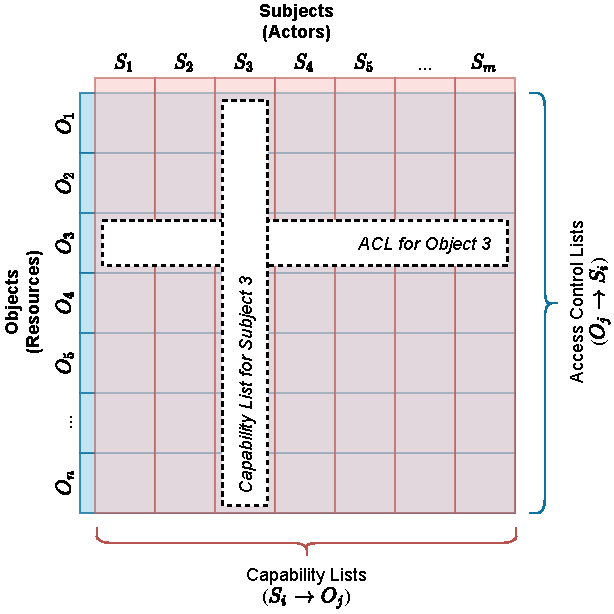
\includegraphics[width=0.8\linewidth]{figs/background/acl.pdf}
  \caption[The access matrix]{
    The access matrix and the relationship between \glspl{acl} and capability
    lists~\cite{anderson1972_report, van_oorschot2020_tools_jewels,
    jaeger2008_os_security}. \glspl{acl} define the set of subjects that have specific
    access rights on a particular object. Capability lists conversely define the access
    rights that a specific subject has on a set of objects. Note that an \gls{acl} may be
    derived by taking the set of all capability lists and vice versa. Taken together,
    these form the access matrix.
  }%
  \label{fig:acl}
\end{figure}

\subsubsection*{The Superuser and Setuid}

To facilitate system administration, many \gls{dac} schemes incorporate the notion of
a \textit{superuser} or \textit{administrator role} into their model. In Unix and
Unix-like operating systems, the superuser or \textit{root} user is denoted by the
\gls{uid} of zero. Any process running with the \gls{euid} of zero is said to be
\textit{root-privileged}. These root-privileged processes can then override the system's
\gls{dac} policy, bypassing permission bits and access control entries on system objects.

In many cases, a program requires additional privileges in order to function. For
instance, a \texttt{login} program would require the ability to read security-sensitive
password entries in \texttt{/etc/shadow}. To achieve such functionality, Unix provides
special \texttt{setuid} and \texttt{setgid} permission bits that implicitly set the
effective user and group IDs of a process to those of the file owner.
A sufficiently-privileged process may also change its own \gls{euid} or \gls{egid} at
runtime using the \texttt{setuid(2)} and \texttt{setgid(2)} family of system calls. The
example login program, for instance, could use these system calls to drop its privileges
to those of the user being logged in. While necessary under the Unix \gls{dac} model,
setuid and setgid binaries have long been the target of exploitation, particularly for
privilege escalation attacks~\cite{dittmer2014_setuid, van_oorschot2020_tools_jewels,
jaeger2008_os_security}.

\subsubsection*{User and Group Assignment}

To alleviate concerns with discretionary access control, systems often take the approach
of assigning a unique user and/or group to a specific application. Such applications are
typically security-sensitive, such as a privileged daemon or network-facing service. This
technique achieves a dual-purpose: firstly, the application can lock down any resources it
owns, simply by restricting any access to its own \gls{uid}; secondly, the resulting
process no longer needs to run under the same \gls{uid} as its parent. This effectively
limits the amount of outside resources that the application can access (so long as
permission bits are correctly configured).

The Android operating system takes this model a step further, assigning a unique \gls{uid}
and \gls{gid} to every application on the system, with optional \gls{uid} sharing between
applications that come from the same vendor. Under this model, no process' \gls{uid} ever
corresponds to a human user. While this arguably improves security, Barrera
\etal~\cite{barrera2012_android} found weaknesses in Android's \gls{uid} sharing model
that can reduce its security to the trustworthiness of an app's signing key.

\subsubsection*{DAC Security Assumptions and Attacks}

Although discretionary access control provides a convenient and intuitive user-centric
model for object ownership and permissions, it makes some dangerous assumptions about
security that can totally invalidate the model in
practice~\cite{shu2016_security_isolation_study}. In particular, \gls{dac} assumes that all
processes are benign and contain no exploitable vulnerabilities. The mere existence off
malware and exploitable vulnerabilities (e.g.\ memory safety vulnerabilities) immediately
invalidates this assumption. For instance, consider an honest but vulnerable piece of
software running under a given \gls{uid} $X$. An attacker exploiting a vulnerability in
this application could perform arbitrary operations on any files owned by $X$. Similarly,
a Trojan horse\footnote{A Trojan horse is a piece of ostensibly benign software that
is designed to perform some malicious action or actions in addition to its ordinary
functionality~\cite{van_oorschot2020_tools_jewels}.}~\cite{shu2016_security_isolation_study,
van_oorschot2020_tools_jewels} can perform arbitrary malicious operations on $X$'s files
without needing to exploit any vulnerability. The fundamental issue with Unix \gls{dac} is
that these files need not necessarily have \textit{anything} to do with the program in
question.

Another fundamental issue with Unix \gls{dac} lies in the ultimate authority of the root
user. Any process running with \gls{euid}=0 is immediately part of the system's
\gls{tcb}\footnote{The \textit{trusted computing base} is the set of all hardware
and software that must be trusted in order for the system to be considered trusted.
Typically, this includes system hardware, the operating system itself, and a small subset
of userspace programs~\cite{jaeger2008_os_security}.}. The same applies to any executable
marked as setuid root. Processes that run with root privileges are prime targets for
attacker exploit, since a successful attack can effectively compromise the entire system.
For instance, confused deputy attacks~\cite{hardy1988_confused_deputy,
shu2016_security_isolation_study} can exploit privileged processes by tricking them into
performing some undesired action. The coarse granularity of Unix \gls{dac} renders it
particularly vulnerable against such attacks.

\subsubsection*{Proposals for Alternative Schemes}

Both industry and academia have long recognized that weaknesses in the Unix discretionary
access control model must be addressed. Many have turned to mandatory access
control~\cite{spencer1999_flask, smalley2001_selinux, wright2002_lsm, cowan2000_apparmor,
schaufler_smack, schreuders2012_towards, hu2013_fsf, harada2004_tomoyo, salaun_landlockio,
singh2019_krsi} (c.f.\ \Cref{ss:mac}) to solve the fundamental issues in \gls{dac}, while
others have proposed improvements or alternative schemes for implementing discretionary
access control~\cite{mao2009_trojan_resistant_dac, solworth2004_layered_dac,
dranger2006_dac_complexity, dittmer2014_setuid, tsafrir2008_setuid, chen2002_setuid}. This
subsection focuses specifically on the latter.

Mao \etal~\cite{mao2009_trojan_resistant_dac} proposed IFEDAC (Information Flow Enhanced
\glsentryshort{dac}) as an alternative \gls{dac} model that is resistant to Trojan horse
attacks.  The insight behind their work was that \gls{dac}'s primary weaknesses lie in the
inability to distinguish requests involving multiple actors. Their mechanism proposes to
track information flows between subjects and use these flows to infer a list of subjects
that have influenced a request.

Under the traditional Unix \gls{dac} model, only the \gls{uid} and \gls{gid} of the
process are considered when making access control decisions; under IFEDAC, the \gls{uid}
and \gls{gid} of the owner of the underlying executable would also be considered, along
with any other parties that may have influenced the state of the running process. This
approach is similar in spirit to taint tracking mechanisms~\cite{livshits2012_dynamic}
(c.f.\ \Cref{ss:taint-tracking}). To enable programs to function correctly, IFEDAC enables
the user to define \textit{exception policy} that specifies exceptions to IFEDAC
enforcement. Mao \etal~recommend that application authors and OS vendors should be
responsible for distributing such policies~\cite{mao2009_trojan_resistant_dac}.

Dranger, Solworth, and Sloan~\cite{solworth2004_layered_dac, dranger2006_dac_complexity}
presented a three-layered model of \gls{dac} mechanisms. The \textit{base layer} defines
the general access control model, while the \textit{parameterization layer} parameterizes
it according to deployment needs.  Finally, the \textit{local initialization layer}
comprises the set of subjects and objects along with their associated protections. The
authors showed that their model was generalizable and that it could be used to implement
any \gls{dac} mechanism.

Dittmer and Tripunitara~\cite{dittmer2014_setuid} examined the implementation and common
usage patterns of the POSIX setuid and setgid \gls{api} across multiple Unix-like operating
systems. They identified weaknesses in systems that do not implement the latest POSIX
standard revisions and suggested that mismatched semantics between various implementors
can be a source of developer error. Finally, they presented an alternative \gls{api} that
partitions \gls{uid} changes into permanent and temporary categories. Tsafrir
\etal~\cite{tsafrir2008_setuid} and Chen \etal~\cite{chen2002_setuid} identified the same
fundamental issues and proposed the adoption of similar mechanisms.


%\subsection{Role-Based Access Control}%
%\label{ss:rbac}
%
%\begin{inprogress}
%  \begin{itemize}
%    \item
%  \end{itemize}
%\end{inprogress}



\section{Extensions to the Unix Security Model}%
\label{s:security-extensions}

Having examined the classical components of an operating system security framework, we now
turn our attention to recent extensions on top of the Unix security model, with
a particular emphasis on Linux and other free and open source Unix-like operating systems.
This section presents a selection of key developments on top of the original Unix security
model which have developed over time, with a particular emphasis on process-level
confinement.

% \begin{inprogress}
%   \begin{itemize}
%     \item The items discussed in 2.1 have been around for a long time
%     \item To solve problems that crop up, this model has been update over time across multiple distributions
%     \item This section presents a selection of key developments to the Unix security model
%   \end{itemize}
% \end{inprogress}

% \todo{Maybe add Grsecurity (OpenWall, etc.) to this background?}

\subsection{POSIX Capabilities}

POSIX capabilities~\cite{posix_capabilities, corbet2006_capabities_a,
corbet2006_capabities_b} are highly related to Unix \gls{dac} in the sense that they were
originally designed to break up the multitude of privileges associated with the
\textit{root} user into more manageable pieces. In this sense, POSIX capabilities (when
properly used) are more conducive to the principle of least-privilege. A process need not
necessarily possess full root-level access to the system when only a small subset of those
privileges are actually required.

Originally specified in the (now withdrawn) 1003.1e POSIX standard, POSIX capabilities
were only ever (partially) implemented on Linux~\cite{anderson2017_comparison}. Other
Unix-like operating systems prefer alternative methods of restricting privileges, many of
which are discussed in \Cref{ss:syscall-filtering}. POSIX capabilities specify three
\textit{capability sets} for a given process: the \textbf{bounding set}, the
\textbf{inheritable set}, and the \textbf{effective set}. The bounding set determines the
set of all capabilities that a process is ever allowed to possess. The inheritable set
determines the set of all capabilities that can be inherited across \texttt{execve} calls.
Finally, the effective set determines the set of capabilities that a process can use
(i.e.\ which capabilities a process currently possesses).

Linux exposes POSIX capabilities through extended filesystem attributes, much the same way
that \glspl{acl} are implemented~\cite{corbet2006_capabities_b}. These file-based
capabilities function in a similar manner to the setuid bit, implicitly setting the
bounding, inheritable, and effective capability sets on execution. In addition so
supporting capabilities as extended filesystem attributes, the kernel also supports
dropping specific capabilities from each of the three sets through the \texttt{ptrctl(2)}
system call. This enables a higher-privileged process (e.g.\ running as root) to drop
elevated privileges while retaining those it needs to function. As of Linux 5.12, the
kernel supports 41 capabilities in total, including the all-encompassing
\texttt{CAP\_SYS\_ADMIN}~\cite{linux_capability_h}.

It is worth mentioning that the term \enquote{POSIX capabilities} does \textit{not}
describe capabilities as they are broadly defined by operating system security
researchers~\cite{anderson2017_comparison}. In particular, Dennis and Van
Horn~\cite{dennis1966_semantics} first defined the notion of capabilities as a means of
restricting access to \textit{pointers}, guarding references to system objects. Unlike the
capabilities defined by Dennis and Van Horn, POSIX capabilities are not associated with
any given system object. Dennis and Van Horn's capabilities more closely resemble that of
the access matrix introduced by Anderson~\cite{anderson1972_report} and similar mechanisms
have been implemented in other systems such as FreeBSD's
Capsicum~\cite{watson2010_capsicum} and the CHERI architecture~\cite{watson2015_cheri,
davis2019_cheriabi}. These are discussed in more detail in \Cref{ss:syscall-filtering}.

\subsection{Mandatory Access Control}%
\label{ss:mac}

In contrast with \gls{dac}, \textit{\gls{mac}} does not delegate permission assignment to
the resource owner~\cite{spencer1999_flask, van_oorschot2020_tools_jewels,
jaeger2008_os_security}. In the context of Unix, this means that \gls{mac} both overrides
traditional discretionary access controls \textit{and} applies access controls to all
users on the system, including root. Historical implementations of \gls{mac} have focused
primarily on \gls{mls}, an access control scheme that revolves around the \textit{secrecy}
of objects and \textit{access level} of subjects~\cite{bell2005_blp}. In a nutshell,
\gls{mls} prevents a subject from reading data with a higher secrecy level or writing data
with a lower secrecy level, preventing breaches in confidentiality and
integrity~\cite{jaeger2008_os_security}.

\subsubsection*{Historical Approaches}

Multics~\cite{vyssotsky1965_multics, corbato1965_multics} was the first operating system
to pioneer the use of an \gls{mls} access control scheme. Memory in Multics was
virtualized into \textit{segments}, each with a \textit{segment descriptor} that outlined
protections that should be applied to that memory. To define an \gls{mls} policy, these
protections included a secrecy level, enforced according to the subjects secrecy level.
These \gls{mls}-style protections were complementary to discretionary \gls{acl}s defined
for every segment along with memory protection rings (the first of their kind), enforced
in hardware~\cite{jaeger2008_os_security}.

While \gls{mls} is primarily applicable to military contexts, \gls{mac} has since evolved
into mainstream use through the advent of alternative implementations. The Flask
microkernel~\cite{spencer1999_flask} introduced a practical architecture for \gls{mac}
policy enforcement that was both scalable and effective. The non-discretionary components
of the Flask security model were hugely influential in the design and implementation of
subsequent \gls{mac} enforcement mechanisms, most notably
SELinux~\cite{smalley2001_selinux, loscocco2001_selinux}.

The basic notion behind flask is straight-forward; the security architecture is divided
into a security server, responsible for storing security policy, and a object manager that
serves requests to userspace applications. When an application requests a resource, the
object manager queries security policy from the security server and decides whether or not
to serve the request based on the resulting enforcement decision. By designing Flask to be
modular in this way, Spencer \etal~achieved a separation of concerns between policy
enforcement and policy decision-making, vital for scalability~\cite{spencer1999_flask,
smalley2001_selinux, loscocco2001_selinux}.

\subsubsection*{Linux Security Modules, SELinux, and AppArmor}

The NSA first introduced SELinux (Security Enhanced Linux)~\cite{smalley2001_selinux,
loscocco2001_selinux} as a Linux kernel patch, with the goal of providing an
implementation of the Flask security architecture~\cite{spencer1999_flask} for the Linux
kernel. Reluctant to restrict users to just one security architecture, the kernel
community eventually agreed that a generic security framework would provide more value
than a single implementation, allowing for multiple upstream security implementations that
could be selected based on the downstream use case. This effort culminated in the
introduction of the \textit{Linux Security Modules} (\gls{lsm})~\cite{wright2002_lsm} framework.

The \gls{lsm} framework consists of a set of security hooks, placed in strategic locations
throughout the kernel~\cite{wright2002_lsm}. Hooks can roughly be divided into
\textit{enforcement} hooks and \textit{bookkeeping} hooks. Enforcement hooks serve as
checkpoints for security enforcement over specific access categories, while bookkeeping
hooks enable a security module to maintain stateful information about subjects and objects
on the system.  \gls{lsm} hooks are not considered to be static, and often change between
kernel versions as new hooks are implemented and both new and existing hooks placed into
various kernel functions~\cite{zhang2021_lsm_file_overhead}. The eventual goal of the
\gls{lsm} framework is to provide complete mediation over kernel security events, however
this is an evolving process and no formal verification exists to prove the security of
\gls{lsm} hooks~\cite{ganapathy2005_lsm}. \Cref{fig:lsm} depicts the basic \gls{lsm} architecture.

\begin{figure}[htbp]
  \centering
  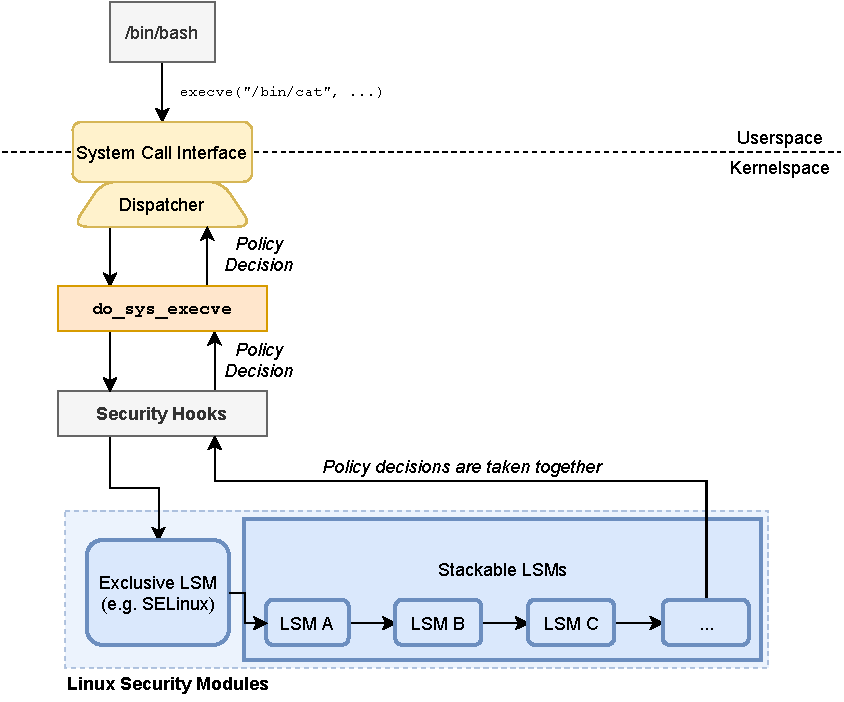
\includegraphics[width=0.8\linewidth]{figs/background/lsm.pdf}
  \caption[The \glsentryshort{lsm} architecture]{
    The \gls{lsm} architecture. A single \textit{exclusive} \gls{lsm} may be loaded at a time,
    and complemented by zero or more \textit{stackable} \gls{lsm}s. When userspace
    requests a privileged operation (e.g.\ through a system call), this operation causes one
    or more security hooks to be invoked. These hooks in turn call into the respective
    hook implementations provided by each loaded \gls{lsm}. Each hook returns a policy
    decision, and these decisions are then taken together to arrive at a final decision.
  }%
  \label{fig:lsm}
\end{figure}

After the introduction of the \gls{lsm} framework, SELinux was refactored into a Linux
security module~\cite{smalley2001_selinux} and subsequently merged into the mainline
kernel. SELinux supports three major types of mandatory access control: (i) role-based
access controls; (ii) type enforcement; and (iii) an optional \gls{mls} policy.
Fundamentally, SELinux policies are based on a notion of subject and object labelling.
A security policy assigns a specific label to subjects and objects, and then specifies
access patterns between these labels.

In an effort to simplify the SELinux policy language, a \textit{reference policy} was
introduced by PeBenito in 2006~\cite{pebenito2006_refpol}, providing a framework for
creating and managing reusable policy templates which can be integrated into new and
existing security policies. SELinux reference policies can be augmented with boolean
options, called \textit{tunables} that provide coarse-grained control over policy
behaviour to system administrators. Sniffen~\cite{sniffen06_guided} implemented a guided
policy generation system that walks application authors through the process of writing
SELinux policy. This framework was further augmented by
MacMillan~\cite{macmillan07_madison}, culminating in the eventual introduction of the
\texttt{audit2allow}~\cite{audit2allow} command line utility for automated policy
generation. Despite these usability improvements, the SELinux policy language is generally
considered to be quite arcane~\cite{schreuders2012_towards}, rendering it difficult for
non-expert users to write and audit security policy.

Since the introduction of SELinux, several alternative \gls{lsm}s have been proposed, many
of which have subsequently been merged into the mainline Linux kernel. AppArmor
(originally called SubDomain)~\cite{cowan2000_apparmor} takes an alternative approach to
SELinux, enforcing security policy based on \textit{pathnames} rather than security
labels.  AppArmor policies, called \textit{profiles}, are assigned on a per-executable
basis. Rather than being labelled, AppArmor policies identify system objects directly
(e.g.\ through pathnames, \gls{ipc} categories, or network \gls{ip} addresses). Each system
object is associated with a particular access pattern, which determines the privileges for
a given AppArmor profile. Similar to SELinux, AppArmor offers a suite of userspace tooling
for automated and semi-automated policy generation based on enforcement
logs~\cite{aa_easyprof, aa_genprof, aa_logprof}.

\subsubsection*{Alternative Linux Security Modules}

Recognizing usability issues in the complexity of SELinux and AppArmor policies,
Schaufler~\cite{schaufler_smack} introduced SMACK (Simplified Mandatory Access Control
Kernel) to offer a simplified label-based enforcement scheme that focuses on expressing
a minimal set of permissions. Like SELinux, SMACK relies on labelling filesystem objects
using extended filesystem attributes. Policies then attach simple access specifiers to
these labels, based on canonical Unix permissions like \texttt{read}, \texttt{write}, and
\texttt{execute}. Some default labels are provided, which grant or revoke blanket
permissions for common tasks such as system daemons or the \texttt{init} process.

Schreuders \etal~\cite{schreuders2012_towards} designed FBAC-LSM (Functionality-Based
Access Control \gls{lsm}) with a similar goal of simplifying policy definition. Unlike
SMACK, which is based on labelling, FBAC-LSM specifies policy in terms of desired
\textit{functionality}. Specifically, FBAC-LSM policies define a set of high-level
functionalities that an application should exhibit. All other functionalities are
prohibited. Schreuders \etal~evaluated FBAC-LSM in terms of its usability and found that
it compares favourably against AppArmor and SELinux~\cite{schreuders2012_towards}.

Hu \etal~\cite{hu2013_fsf} proposed FSF (File System Firewall), which applies
firewall-like semantics to filesystem objects. Their goal was to create a more usable,
file-specific access control mechanism. FSF policies are defined in policy files,
comprised of simple rules that specify a file along with some combination of
\texttt{read}, \texttt{write}, and \texttt{execute} access. \textit{Redirection rules} are
primary differentiating factor between FSF and conventional file-based access controls.
Taking inspiration from similar functionality in network firewalls, a redirection rule can
be used to convert one file access into another, transparently to the target application.
Hu \etal~conducted a user study comparing their prototype to Unix \gls{dac} and SELinux
and found that FSF performed favourably in policy comprehensibility and accuracy.

The TOMOYO~\cite{harada2004_tomoyo} \gls{lsm} takes an alternative approach, emphasizing
policy generation and building generation functionality into the \gls{lsm} directly.
Rather than involving userspace helpers, TOMOYO generates policy by inferring
per-application profiles through the \gls{lsm} hooks they invoke. Programs can
additionally discard their privileges through a TOMOYO-specific system call, similar to
the notion of dropping privileges under the POSIX capabilities model. Like AppArmor,
TOMOYO relies on pathnames to identify resources rather than assigning security labels.
Users have the option to edit generated policies as required, but the intent is to require
as little user involvement as possible~\cite{harada2004_tomoyo}.

The Landlock~\cite{salaun_landlockio, salaun_landlock_patch} \gls{lsm} was recently
introduced into the mainline Linux kernel as a contemporary alternative to
\texttt{seccomp(2)} (covered in \Cref{sss:seccomp}). Landlock was originally intended to
allow unprivileged userspace processes to load highly restricted \gls{ebpf} programs into
the kernel to define security filtering logic~\cite{salaun_landlock_patch}. However, due
to concerns related to the security of unprivileged \gls{ebpf}, this functionality was
later reworked into a set of simple access rules and no longer has any association with
\gls{ebpf}~\cite{salaun_landlockio}. Under Landlock, a process creates a \textit{ruleset}
using the \texttt{landlock\_create\_ruleset(2)} system call, adds rules to that ruleset,
then confines itself by committing to that ruleset. Developers may add this confinement
logic directly into their software or may write specialized userspace wrappers to apply
generic confinement to applications.

Singh~\cite{singh2019_krsi} introduced the KRSI (Kernel Runtime Security Instrumentation)
framework for attaching \gls{ebpf} programs to \gls{lsm} hooks with the goal of defining
dynamic audit and policy enforcement filters. While similar in spirit to the original
Landlock proposal~\cite{salaun_landlock_patch}, KRSI differs fundamentally in that it
remains a \textit{privileged} \gls{lsm}; only root-privileged processes may load
\gls{ebpf} \gls{lsm} programs into the kernel. \bpfcontain{} and \bpfbox{} are both based
on the KRSI framework. \Cref{ss:bpf-programs-bg} examines the KRSI framework in more
detail.

%Radhakrishnan~\cite{radhakrishnan2006_kernelsec} \todo{DESCRIBE THIS OR DROP IT}



\subsection{System Call Filtering and Capabilities}%
\label{ss:syscall-filtering}

Since system calls define the canonical interface for communication between userspace
processes and the operating system kernel~\cite{jaeger2008_os_security}, they are
a natural fit for defining the protection interface of a confinement mechanism. In
particular, \textit{system call filtering} is a widely-used technique for application
sandboxing and self-confinement~\cite{anderson2017_comparison}. Indeed, \gls{lsm}s,
covered in the previous section, can be thought of as a form of system call filtering,
although security hooks are placed manually within system call implementations and do not
necessarily conform to the same semantics as the underlying system
calls~\cite{wright2002_lsm}.

Related to this notion of system call filtering are \textit{capabilities}\footnote{Here,
the term \enquote{capabilities} is a disparate term from \enquote{POSIX capabilities,} covered in
\Cref{ss:dac}.}, which guard access to a particular reference, associating privileges with
a handle to a given object on the system. For instance, the \texttt{open(2)} system call
returns a \textit{file descriptor}, which constitutes a reference to a particular
filesystem object. A capability associated with this file descriptor would then restrict
subsequent operations on the file descriptor, effectively restricting access to the
underlying file.

\subsubsection*{System Call Tracing}
\label{sss:ptrace}

In Unix, ptrace~\cite{ptrace, padala2002_ptrace} (short for process trace) is a mechanism
provided by the kernel that allows one process (the tracer) to attach itself to another
(the tracee), tracing and possibly manipulating nearly any aspect of its execution, system
calls, memory, and registers. Originally designed as a debugging interface~\cite{ptrace,
padala2002_ptrace}, ptrace has also been applied to implement system call
filtering~\cite{goldberg96_janus, wagner1999_janus, jain2000_filtering}. However, ptrace
has fallen out of favour, particularly in production use cases, due to its immensely high
overhead (on the order of several thousand percent~\cite{zinke2009_overhead}) and
propensity to introduce undefined behaviour when tracing even moderately complex
software~\cite{swiecki2017_promises}. Due to its invasive nature, a tracer process must
either be the direct parent of a tracee or must have sufficient privileges to trace the
child process\,---\,on Linux, this translates to either the \texttt{CAP\_SYS\_PTRACE}
capability or the all-encompassing \texttt{CAP\_SYS\_ADMIN}.

Janus~\cite{goldberg96_janus, wagner1999_janus} was an early exploration of how
\texttt{ptrace} could be applied to confine applications by filtering system calls.  The
original Janus prototype was designed for Oracle Solaris using its ptrace interface,
exposed through the \texttt{procfs} virtual filesystem~\cite{goldberg96_janus}.
A subsequent port of Janus was released for Linux~\cite{wagner1999_janus}, although it
required invasive modifications to Linux's ptrace implementation, dubbed ptrace++ by the
authors. Janus worked by attaching to the target process using ptrace, then tracing system
calls made by the target process and categorizing them into groups based on functionality.
A Janus policy could allow or deny specific categories of system call, confining the
application in a coarse-grained manner. The tracer process, called the \textit{supervisor
process}, would then be able to kill the offending process or inject failure into the
offending system call when it detected a policy violation.  Jain and
Sekar~\cite{jain2000_filtering} implemented a similar system call monitor, adding the
ability to modify system call arguments and using a different policy language design.

Provos' Systrace~\cite{provos2003_systrace} uses ptrace to analyze per-process system
calls and generate a system-call-level policy. Unlike Janus~\cite{goldberg96_janus,
wagner1999_janus} and Jain~\etal~\cite{jain2000_filtering}, Systrace supports intrusion
detection, policy generation, and audit logging, providing a mechanism to automatically
analyze process behaviour. Systrace also supports one highly unconventional feature, which
Provos calls \textit{privilege elevation}. The notion behind privilege elevation is to
allow a program to escalate its privileges selectively for specific system call access
patterns, preventing the need for coarse-grained privilege escalation such as setuid root.

Forrest, Somayaji, and Hofmeyr~\cite{forrest1996_sense_of_self} implement an intrusion
detection system, pH (process Homeostasis), based on system call sequences, although it
does not rely on ptrace and analyzes system call sequences instead of individual call
patterns. Rather than as a confinement solution, pH was strictly designed as a behavioural
anomaly detection system, although this approaches confinement as profile accuracy
improves.  Findlay~\cite{findlay2020_ebph} (the author of this thesis) later ported pH to
use \gls{ebpf} to analyze system call sequences.

\subsubsection*{OpenBSD Pledge and Unveil}
\label{sss:pledge}

OpenBSD's \texttt{pledge(2)} and \texttt{unveil(2)} system calls form the backbone of its
built-in sandboxing framework. A pledge~\cite{pledge} consists of a list of
\textit{promises}, high-level descriptions of what behaviours a program expects to exhibit
in the future, similar in spirit to Janus' high-level categories~\cite{goldberg96_janus,
wagner1999_janus}. The pledge system call takes two space-separated lists of promises, one
to be applied immediately and another to be applied upon making an \texttt{execve(2)}
call. To prevent privilege escalation, subsequent calls to \texttt{pledge(2)} take the
union of existing promises and new promises, precluding a process from escaping its
initial bounding set~\cite{pledge}.

Promises vary in granularity; the most coarse-grained promise, \texttt{stdio}, allows
a total of 69 distinct system calls, enabling the full suite of C standard library
stdio-family calls. Others, like \texttt{chown}, are more conservative, enabling only one
(albeit in this case very powerful) system call. In total, \texttt{pledge(2)} includes 33
distinct promises, as of OpenBSD 6.9~\cite{pledge}. Due to its coarse granularity and lack
of concern for specific system objects, pledge has been criticized as being
overly-permissive~\cite{anderson2017_comparison}.

Unlike pledge, \texttt{unveil(2)}~\cite{unveil, corbet2018_unveil} operates on specific
filesystem paths, making a promise about the kinds of operations the process will perform
on file descriptors associated with these paths. Specifically, unveil is concerned with
four kinds of permissions: read, write, execute, and create/delete. Unveiling a directory
unveils all files and directories underneath, recursively. Although this approach is
finer-grained than pledge, it is file-specific and offers a trade-off between granularity
and usability. The official manual page for unveil~\cite{unveil} recommends that
developers use it at the granularity of directories, despite the fact that this may result
in overpermission in practice. For instance, consider a hard link to the root of the
filesystem placed by an attacker within some unveiled directory. The unveiling process
would now have full access to the entire filesystem, constituting a sandbox escape.

\subsubsection*{Linux Seccomp and Seccomp-bpf}%
\label{sss:seccomp}

In Linux, the primary facility for direct system call filtering is
\texttt{seccomp(2)}~\cite{anderson2017_comparison, seccomp, prctl, edge2015_seccomp}.
Unlike OpenBSD's pledge and unveil~\cite{pledge, unveil}, seccomp filters directly over
system calls, without any blanket categorization. Initially, seccomp was highly limited,
restricting a process to only four system calls: \texttt{read(2)} and \texttt{write(2)}
for reading and writing open file descriptors, \texttt{sigreturn(2)} for handling signals,
and \texttt{exit(2)} to enable self-termination. Using any other system call would result
in an immediate SIGKILL delivered from the kernel, forcefully ending the offending
process.

Later, seccomp was extended to enable processes to define custom allowlists, denylists,
and enforcement actions using classic \gls{bpf} filters~\cite{edge2015_seccomp}. This new
incarnation was dubbed seccomp-bpf. While allowing for much finer-grained confinement
policy than pledge and unveil, seccomp-bpf has its own limitations which can result in
ineffective (and possibly dangerous) policies. In seccomp-bpf, filters are defined over
system call numbers and (optionally) arguments. Unless the developer takes great care to
correlate system call numbers with the specific target architecture, the resulting policy
may allow and deny incorrect system calls, resulting in broken policies that break
applications in the best case and expose security vulnerabilities in the worst case.

Another innate problem with seccomp arises due to its fine-granularity. Paradoxically,
avoiding system call categorization can expose vulnerabilities, due to system call
equivalence classes. For instance, the \texttt{openat(2)} system call can perform the same
functionality as the \texttt{open(2)} system call, with slightly different \gls{api} semantics.
A seccomp-bpf filter allowing one system call but denying the other is now totally broken
and vulnerable to sandbox escape.  Similarly, argument checking on pathnames or file
descriptors can be vulnerable to \gls{toctou} race conditions in practice, rendering such
policies ineffective~\cite{anderson2017_comparison}.

A final consideration for seccomp-bpf is that the development of seccomp-bpf policies
requires knowledge of the relatively arcane \gls{cbpf} syntax. This problem is somewhat
alleviated by the existence of library wrappers~\cite{libseccomp} around seccomp-bpf
functionality, although the usability of these solutions remains somewhat questionable,
particularly given the many pitfalls of seccomp-bpf policy
authorship~\cite{anderson2017_comparison}.

\subsubsection*{FreeBSD Capsicum and CHERI Capabilities}
\label{sss:capsicum}

Unlike the system call filters presented earlier in this section, FreeBSD's
\texttt{capsicum(2)} \cite{watson2010_capsicum, anderson2017_comparison} is a true
implementation of capabilities as they were originally described by Dennis and Van
Horn~\cite{dennis1966_semantics}. Specifically, capsicum capabilities are an extension on
top of Unix file descriptors, the canonical reference to files and file-like objects such
as network sockets and character devices. Capsicum adds an unforgeable access token to
each file descriptor, granting the corresponding process specific access rights over that
file descriptor. Whereas alternatives like seccomp-bpf~\cite{seccomp} and
pledge~\cite{pledge} restrict access at the system-call-level, capsicum restricts access
at the resource-level and enforces this access within the system call layer.

To confine processes, capsicum exposes a special \texttt{cap\_enter(2)} system call which
causes a process to enter \textit{capability mode}. A process in capability mode no longer
has access to global namespaces (e.g.\ the \gls{pid} namespace) and may only make a subset of
system calls which do not directly access these global namespaces. Other system calls are
constrained so that they may only operate under the context of an open capability
descriptor (a file descriptor which has been extended with capability
information)~\cite{watson2010_capsicum}. The end-result is an expressive and fine-grained
self-confinement framework for FreeBSD applications, which comes at a small usability cost
compared with coarser-grained alternatives like \texttt{pledge(2)}~\cite{pledge}.

In 2015, Watson \etal~designed CHERI~\cite{watson2015_cheri} as an extension to the MIPS
\gls{isa} enabling the capability-based protection of memory pages. Under CHERI, the
operating system kernel and userspace runtime extend the traditional memory model with
capabilities using the CHERI \gls{isa}. This enables generic capability-based protection at
the level of memory pages. While powerful, this extension requires dedicated hardware
support. Watson \etal~implemented their prototype on an \gls{fpga}~\cite{watson2015_cheri}
and later extended the FreeBSD \gls{abi} to work with CHERI capabilities~\cite{davis2019_cheriabi}.



\subsection{Taint Tracking}%
\label{ss:taint-tracking}

\textit{Taint tracking}~\cite{livshits2012_dynamic} describes the notion of tracking
changes to memory containing application data as it is mutated, copied, and moved by the
underlying application. Such data is considered \textit{tainted} when it is modified by
some external source in such a way as the data can no longer be trusted.  For instance,
a buffer might be populated by an external network connection or local user input. The
security benefits of such a mechanism are obvious. An active attack requires some user
input into a program in order to exploit a vulnerability; by tracking untrusted user input
and treating it as untrusted, developers can avoid attacker exploitation of sensitive code
paths. Beginning with Perl's \textit{taint mode}~\cite{hurst2004_perl}, taint tracking has
enjoyed a rich body of literature~\cite{livshits2012_dynamic, conti2010_taint,
bello2012_taint, ermolinskiy2010_towards, zavou2011_taint, yin2007_panorama,
zhu2011_taint_eraser, cheng2006_taint, clause2007_taint, chin2009_efficient} since its
inception.

In Perl's taint mode~\cite{hurst2004_perl}, a special command line flag triggers the
interpreter to flag untrusted user input and prevent it from being passed as input to
functions explicitly marked as \textit{unsafe}. To circumvent this restriction,
a developer could perform a pre-determined set of sanity checks on the data to
\textit{untaint} it. Rather than acting as an outright security mechanism, the goal was to
encourage developers to take care in processing untrusted data. Incorrect or insufficient
sanity checks on the data or running the Perl interpreter without the taint flag would
result in no additional security benefits whatsoever. After Perl, similar taint tracking
mechanisms have been added to other interpreters and language runtimes, including Ruby,
PHP, and Python~\cite{conti2010_taint}.

Conti, Bello, and Russo~\cite{conti2010_taint, bello2012_taint} implemented more advanced
taint tracking functionality for the Python programming language as a library that
developers could use directly. Their argument was that implementing such a taint mechanism
at the language-level rather than at the interpreter-level could enrich the traditional
taint-tracking approach with use-case-specific metadata and facilitate extensions to
support complex data types.

With the goal of creating a generic and reusable taint tracking mechanism, several
researchers have proposed application-transparent taint tracking. Many have turned to
virtualization or emulation runtimes~\cite{ermolinskiy2010_towards, zavou2011_taint,
yin2007_panorama} such as QEMU, KVM, or Xen, using built-in introspection features to
track the propagation of data within (and even between) running processes. Others have
proposed the adoption of static analysis or library
instrumentation~\cite{zhu2011_taint_eraser, cheng2006_taint, clause2007_taint} techniques
to reduce overhead and eliminate the need to run applications under expensive
virtualization monitors. Others have built taint tracking logic into existing language
runtimes, such as the Java Virtual Machine~\cite{chin2009_efficient}.



\section{Process-Level Virtualization}%
\label{s:virtualization}

We now step away from \textit{confinement} to focus on process-level
\textit{virtualization} primitives employed in Unix-like operating systems. Whereas
confinement primitives have the goal of restricting a process' behaviour, virtualization
primitives instead limit the process' ability to see the world around it. This property
should not be confused with \textit{isolation}. True isolation requires a mixture of both
virtualization and confinement mechanisms to restrict access to system resources and
prevent unwanted behaviour.

\subsubsection*{Chroots and Chroot Jails}

To virtualize the filesystem, Unix has classically supported the \texttt{chroot(2)} system
call~\cite{mcfearin2011_chroot_jails}, used to change the filesystem root (\texttt{'/'})
to some directory, specified as an argument. From the process' point of view, this
directory becomes its new filesystem root. However, chroot suffers from several issues
that render it totally ineffective as a security mechanism. Chroot escapes, path
traversals, spurious access to special filesystems and devices, and superuser privileges
all totally invalidate chroot as an isolation mechanism~\cite{mcfearin2011_chroot_jails}.

For instance, consider a call to \texttt{chroot("/my/new/root")}. Without a follow-up call
to \texttt{chdir(2)} to change the process' current working directory, a simple call to
\texttt{chdir("..")} is enough to escape the chroot jail. Even with the aforementioned
precautions, a process that has or is able to obtain superuser privileges can simply
create a new directory, re-invoke chroot, and perform the same escape as
before~\cite{mcfearin2011_chroot_jails}. Without the proper confinement mechanisms and
necessary precautions to prevent such escapes, chroot cannot be considered an effective
isolation technique. In fact, chroot escapes have been a source of many vulnerabilities
with container management engines like Docker in the past~\cite{combe2016_to_docker}.
McFearin~\cite{mcfearin2011_chroot_jails} proposed updates to the POSIX standard that fix
many of chroot's security flaws, but these have not been adopted.

\subsubsection*{FreeBSD Jails and Solaris Zones}

Kamp \etal~\cite{kamp2000_jails} presented FreeBSD's \texttt{jail(2)} as a more secure
alternative to \texttt{chroot(2)} jails. In particular, the jail system call is a heavily
extended wrapper around FreeBSD's chroot implementation. A call to jail begins by
allocating and populating a \texttt{prison} data structure that maintains metadata related
to the jailed process group, and finishes by simply invoking the standard chroot
implementation. Unlike chroot, Jails take care to avoid the standard pitfalls that may
result in a chroot escape and heavily limit the privileges of the root user within the
jail. In this respect, the jail system call can be seen as a hybrid between
a virtualization and confinement mechanism, approaching a full solution.

Jails take the approach of defining a clear security boundary around a collection of
processes, filesystem resources, and network resources~\cite{kamp2000_jails}. A process
existing within this boundary (i.e.\ a member of the jail) enjoys the standard set of Unix
permissions on resources within the jail. Access to resources outside of the jail is
forbidden, including access by the root user. Visibility is similarly restricted by
remapping namespaces in such a way as outside resources are effectively invisible.
Defining a clear protection boundary enables the jail to enforce sensible security policy
without burdening the administrator with the details of writing such
a policy~\cite{kamp2000_jails}.

Solaris Zones~\cite{price2004_zones} later arose as a commercial solution for
process-level virtualization. The goal was to implement namespace remapping and security
isolation for commercial server deployments in (possibly multi-tenant) Solaris
environments. The implementation details of Solaris' Zones are similar to those of
FreeBSD's Jails; a per-task data structure manages the associate between tasks and Zones,
allowing the kernel to perform the necessary remapping and security checks.

\subsubsection*{Linux Namespaces and Cgroups}

Unlike FreeBSD~\cite{kamp2000_jails} and Solaris~\cite{price2004_zones}, Linux takes
a different approach to process-level virtualization. In particular, Linux's
virtualization strategy consists of two separate mechanisms, \textit{namespaces} and
\textit{cgroups} (short for process control groups). These mechanisms, in turn, can be
further subdivided into specific types, targeting different kinds of system resources.
Notably, namespaces and cgroups are \textit{not} confinement mechanisms in and of
themselves. This property is in stark contrast with Jails and Zones, which were designed
to offer strong confinement guarantees over their respective security boundaries.
As the canonical process-level virtualization building blocks in Linux, namespaces and
cgroups form the backbone of Linux containers (c.f.\ \Cref{ss:container-security-bg}).

Linux namespaces~\cite{biederman2006_namespaces, linux_namespaces} limit the visibility of
system resource by providing a virtual remapping of global resource identifiers to
a process or process group. Such identifiers include process IDs, user IDs, filesystem
mounts, \gls{ipc} objects, and network interfaces, among others. Linux supports namespace
creation and entry via the \texttt{clone(2)} and \texttt{unshare(2)} system calls, for
isolating child processes and existing processes respectively. As of version 5.13, the
Linux kernel supports eight distinct namespaces, depicted in \Cref{tab:namespaces}. Other
namespaces have been proposed and/or planned for inclusion, including a security
namespace~\cite{sun2018_security_namespace} for virtualizing \gls{lsm} hooks.

\begin{table}
\begin{tabular}{lp{3in}}
    \toprule
    Namespace & Isolates \\
    \midrule
    \multirow{1}{*}{\glsentryshort{pid}} & \glspl{pid}\\
    \multirow{1}{*}{Mount} & Filesystem mountpoints\\
    \multirow{1}{*}{Net} & Networking stack\\
    \multirow{1}{*}{\glsentryshort{uts}} & Host and domain names\\
    \multirow{1}{*}{\glsentryshort{ipc}} & Inter-process communication objects\\
    \multirow{1}{*}{User} & \glspl{uid} and \glspl{gid}\\
    \multirow{1}{*}{Time} & System time\\
    \multirow{1}{*}{Cgroup} & Cgroup membership\\
    \bottomrule
\end{tabular}
\caption[Linux namespaces]{
  Linux namespaces (as of kernel version 5.13) and what they can be used to isolate~\cite{linux_namespaces}.
}
\label{tab:namespaces}
\end{table}

Complementary to namespaces, cgroups~\cite{cgroups, gao2019_houdini} divide processes into hierarchical
groups, performing resource accounting and restricting access to quantifiable resources
such as memory, \gls{cpu} clock cycles, block I/O, and device drivers. From a security
perspective, such restrictions are useful to prevent resource starvation attacks against
the host. However, Gao \etal~\cite{gao2019_houdini} found that this protection is
incomplete and often misleading, allowing up to 200$\times$ the allotted resource limits
by exploiting out-of-band resource consumption techniques. To interact with the cgroup hierarchy,
Linux exposes a virtual filesystem which encodes cgroup membership in its directory structure.
Cgroup membership visibility can be virtualized using the cgroup namespace~\cite{cgroups}.



\section{Containers and Virtual Machines}%
\label{s:containers-bg}

%This section introduces the concept of containers, examines how they compare with
%alternatives like hypervisor-based virtual machines, discusses the area of container
%security, and surveys related work in the container security space.

Classically, virtualization of a system has been accomplished by means of
a hypervisor~\cite{eder2016_hypervisor_container, sultan2019_container_security}.
Hypervisors implement an interface which overlays the underlying system hardware,
enabling one or more \textit{guest operating systems} to be installed on a single physical
host. These guest systems are then called \textit{virtual machines}. Due to the level of
indirection provided by the hypervisor and the guest operating system kernel, virtual
machines are generally considered to be quite \textit{strongly isolated} from each other,
but this isolation comes at the cost of much higher overhead, both in terms of storage and
performance~\cite{eder2016_hypervisor_container, sultan2019_container_security}.
\Cref{s:cp-rethinking} in \Cref{c:confinement-problem} discusses the differences between
virtual machines and containers in more detail and addresses some common misconceptions
about the levels of isolation they provide.

%Hypervisors can be classified into one of two types, depending on how they are deployed
%and implemented.  Type I hypervisors are implemented directly on top of hardware, whereas
%type II hypervisors run on top of a host operating system. This results in a further layer
%of indirection between the guest and the system hardware and thus a further degradation in
%performance.

% \todo{With HVMs, the security comes from the virtualization, well-defined barrier from one
% machine to another, opt in to whatever is going to cross it}

\textit{Containers} have emerged as a new unit of computation in recent years, providing
a lighter-weight alternative to full hypervisor-based
virtualization~\cite{sultan2019_container_security, eder2016_hypervisor_container}.
Unlike virtual machines, containers run directly on the host operating system, rather than
directly atop a hypervisor, and share the host operating system kernel with each other and
with ordinary host processes. In fact, a container is nothing more than a discrete
collection of processes (sometimes only one process) that share some common isolation from
the rest of the system by way of virtualization and confinement primitives. These
primitives typically include namespaces and cgroups, along with optional confinement
mechanisms like seccomp-\gls{bpf} and Linux \gls{mac} policy. Since they directly share
the host \gls{os} kernel and do not require a guest operating system, containers are
significantly lighter-weight and more performant than virtual machines, but at the cost of
weaker base isolation. \Cref{fig:virt} depicts the major differences between container and
hypervisor-based architectures.

% \begin{figure}[tbp]
%   \centering
%   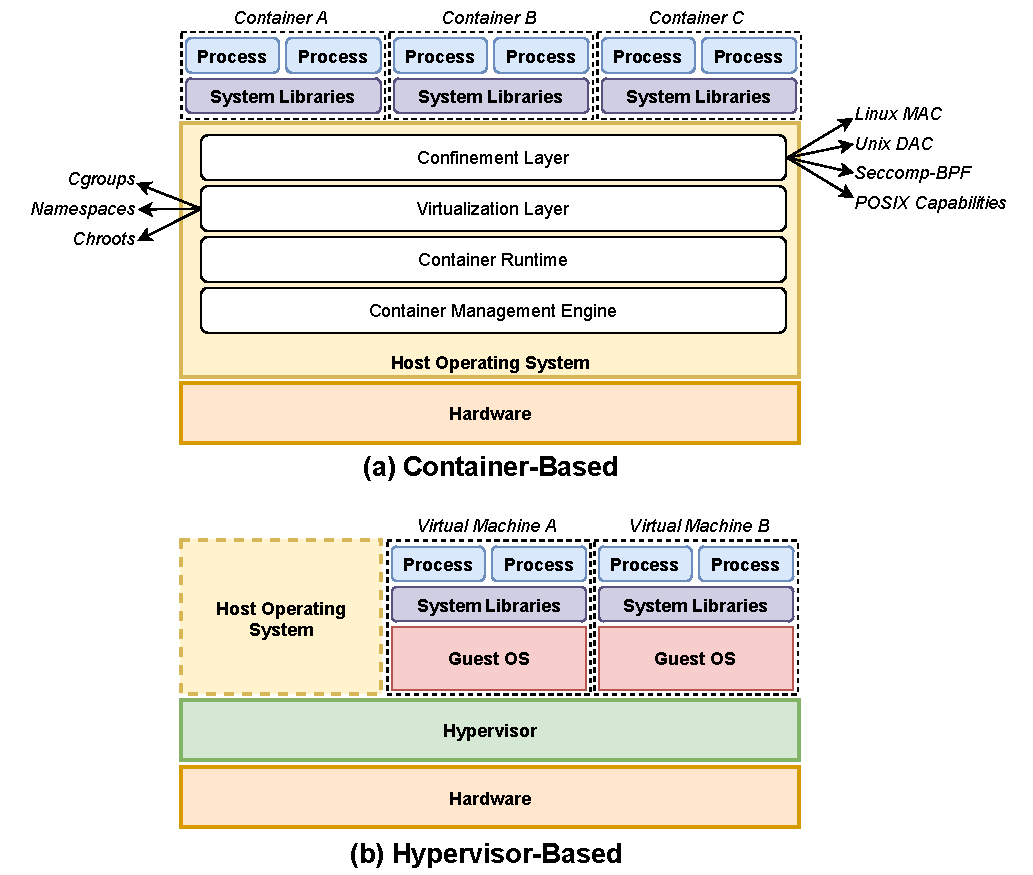
\includegraphics[width=0.8\linewidth]{figs/background/virtualization.pdf}
%   \caption[A comparison of virtual machine and container architectures]{
%     A comparison of virtual machine and container
%     architectures~\cite{sultan2019_container_security, eder2016_hypervisor_container}.
%     Containers \textbf{(a)} achieve virtualization using a thin layer provided by the host
%     \gls{os} itself. They share the underlying operating system kernel and resources,
%     requiring no guest \gls{os}. Type I hypervisors \textbf{(b)} virtualize and control
%     the underlying hardware directly, but require full guest operating systems on top of
%     the virtualization layer. Type II hypervisors \textbf{(c)} run on top of a host
%     operating system but still require full guest operating systems above the
%     virtualization layer.
%   }%
%   \label{fig:virt}
% \end{figure}

\begin{figure}[htbp]
  \centering
  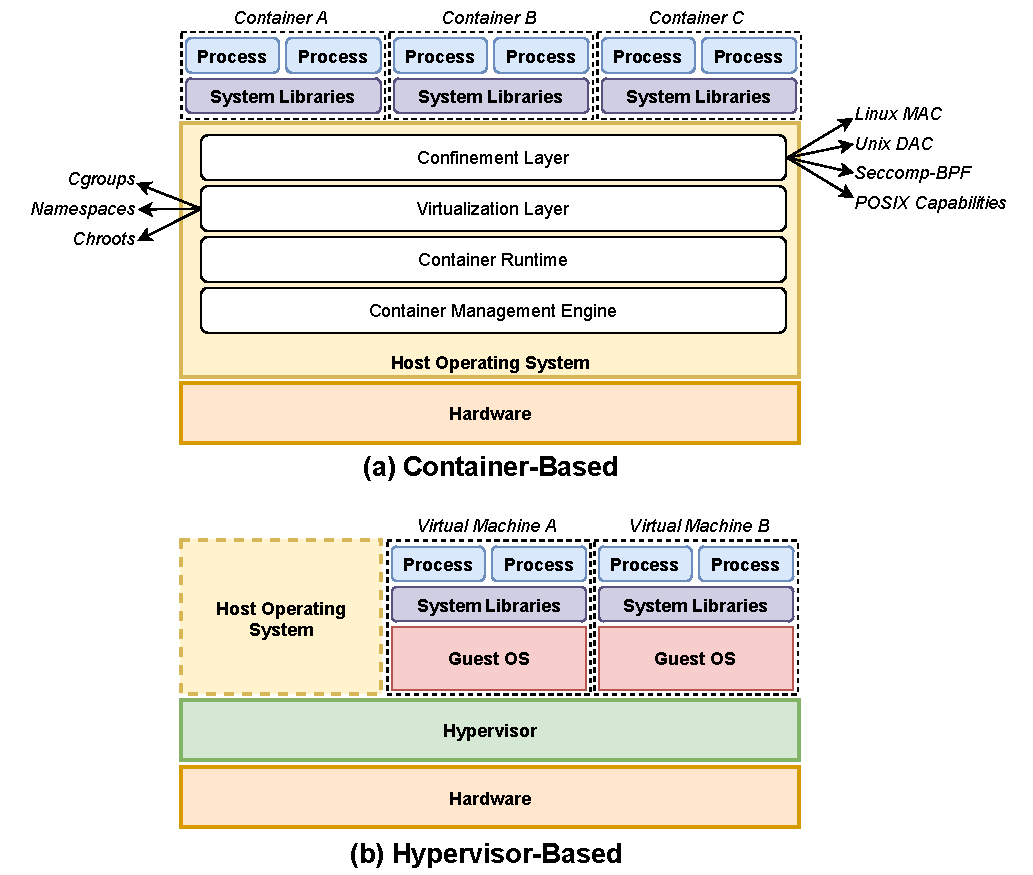
\includegraphics[width=1\linewidth]{figs/background/virtualization.pdf}
  \caption[A comparison of virtual machine and container architectures]{
    A comparison of virtual machine and container
    architectures~\cite{sultan2019_container_security, eder2016_hypervisor_container}.
    Containers \textbf{(a)} achieve virtualization using a thin layer provided by the host
    \gls{os} itself. They share the underlying operating system kernel and resources,
    requiring no guest \gls{os}. A hypervisor \textbf{(b)} virtualizes and controls the
    underlying hardware directly, but requires full guest operating systems on top of the
    virtualization layer.
  }%
  \label{fig:virt}
\end{figure}

% \begin{table}[htbp]
%   \centering
%   \caption[A high-level comparison of hypervisors and containers]{
%     A high-level comparison of hypervisors and containers. \fullc{} means property fully
%     satisfied; \halfc{} means property somewhat satisfied; and \emptyc{} means property
%     not satisfied.
%   }%
%   \label{tab:virt-comparison}
%   \begin{tabular}{lllcccp{1.6em}}
%   \toprule
%   & Deployment & Implementation & \rot{60}{1.6em}{Host-Isolated} & \rot{60}{1.6em}{Light-Weight} & \rot{60}{1.6em}{High-Performance} & \\
%   \midrule
%   Type I \glsentryshort{vm}  & Hardware & Guest \glsentryshort{os} & \fullc  & \halfc  & \halfc  & \\
%   Type II \glsentryshort{vm} & Host OS  & Guest \glsentryshort{os} & \halfc  & \emptyc & \emptyc & \\
%   Containers                 & Host OS  & Namespaces + Cgroups     & \emptyc & \fullc  & \fullc  & \\
%   \bottomrule
%   \end{tabular}
% \end{table}

\subsection{Container Security}%
\label{ss:container-security-bg}

Due to the nature of containers as specialized process groups, any notion of container
security is necessarily tightly coupled with the underlying security primitives exposed by
the host operating system. These include the virtualization primitives discussed in
\Cref{s:virtualization}, and the confinement primitives discussed in
\Cref{s:process-security-model,s:security-extensions}. Whereas the primary attack surface
of a virtual machine is comprised of the interface exposed on top of hardware, the attack
surface of a container is comprised of the system calls that it uses to interact with the
host operating system kernel. Every system call is an opportunity to exploit a kernel
vulnerability; over-zealous resource-sharing is an opportunity to establish a covert
channel, or perform a confused deputy attack~\cite{hardy1988_confused_deputy} against
a privileged application. The cost to mount such attacks rapidly decreases as isolation
from the host operating system decreases.

% While containers are lighter-weight than virtual machines, they are necessarily less
% secure, since they share and interact directly with the host operating system kernel.
% Although hypervisor escapes are not unheard of~\cite{dubrelle2015_hypervisor,
% eder2016_hypervisor_container}, they are far less common than container escapes,
% particularly given the fact that variabilities in container configuration can easily
% introduce holes in confinement~\cite{sultan2019_container_security}. Rather than going
% through a hypervisor (either directly to hardware or to a subsequent system call),
% containers directly make system calls to the host kernel. Not only does this make the
% probability of container escape more likely, but it also increases the host-to-container
% and container-to-host attack surface.

\begin{inprogress}
  \begin{itemize}
    \item Container exploits vulnerability in the kernel
    \item Container exploits vulnerability in the host configuration
    \item Container exploits vulnerability in a host process
  \end{itemize}
\end{inprogress}

\Cref{fig:containersec} depicts a high-level threat model for containers from the
perspective of the host operating system. \todo{Connect each part of the figure to the
text.} This model comprises a number of attack vectors, each targeting a different part of
the system. A malicious container can target another container, a regular host process, or
the host operating system kernel. Similarly, a malicious host process can target
a container. To attack the \gls{os} kernel, a container must generally exploit
a kernel-level vulnerability, such as a memory safety error in a system call
implementation. To mitigate such attacks, the attack surface exposed by the kernel to the
container should be minimal. Other classes of attack rely on exploiting the intended
effects of system calls for in unintended ways.  For instance, a misconfigured security
policy might allow a containerized process to load a kernel module or perform inter-process
communication with an external daemon. Abusing shared resources can have a similar affect,
allowing a container to manipulate or tamper with an external process.

\begin{figure}[htbp]
  \centering
  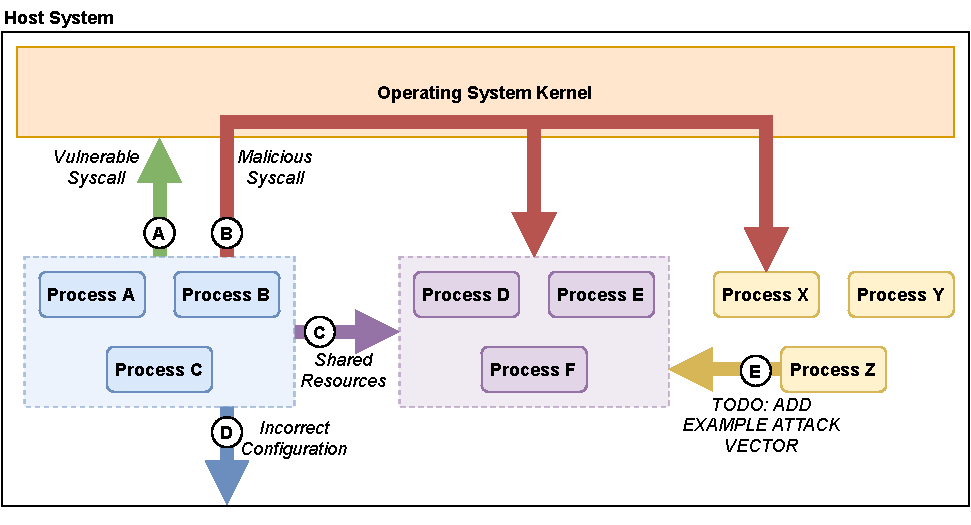
\includegraphics[width=0.8\linewidth]{figs/background/container_security.pdf}
  \caption[A sample threat model for container security]{
    A sample threat model for container security.
    \todo{Description here}
  }%
  \label{fig:containersec}
\end{figure}

\todo{Add a bulleted list of container escapes}
\begin{inprogress}
\begin{itemize}
  \item It's kind of leaky
  \item Even if you configure it perfectly, there are ways to misconfigure it
  \item The things you are subject to are the things you're subject to in the classic security model
  \item No different than software security in general... Because a container is just a set of processes
\end{itemize}
  \begin{itemize}
    \item Shared-resource attack
    \item Privilege escalation
    \begin{itemize}
      \item Exploiting a privileged process (e.g.\ confused deputy)
      \item Exploiting kernel directly
    \end{itemize}
  \end{itemize}
\end{inprogress}

\subsubsection{Container Security in Industry}%
\label{sss:container-security-industry}

Existing container security on Linux is supported by a number of fundamental
virtualization and confinement mechanisms, covered in \Cref{s:process-security-model} and
\Cref{s:security-extensions}. Namespaces virtualize and limit the visibility of global
resource identifiers and cgroups virtualize and limit the available quantities of system
resources. Dropped POSIX capabilities allow the container to partition coarse-grained root
privileges into finer components. Seccomp-bpf filters limit the availability of system
calls to the container, while Linux \gls{mac} policies, enforced by an \gls{lsm} restrict
the container's access to system resources. Unix \gls{dac}, possibly accompanied by a new
user namespace, can limit the container's access as well, when properly configured.

\gls{lxc}~\cite{lxc_security} is a container runtime for Linux that directly exposes
low-level virtualization and confinement primitives. \gls{lxc} exposes namespaces and
cgroups to virtualize system resources and seccomp-bpf to filter system calls, reducing
the kernel's attack surface.

Docker~\cite{docker_security, bui2015_docker_analysis, combe2016_to_docker}, originally
based on \gls{lxc}, provides a high-level interface for creating, manipulating, and
running container images. Docker places containers in a new cgroup with sensible defaults
for resource virtualization. To isolate processes, the filesytem, and network interfaces,
Docker containers run in a new \gls{pid}, \gls{ipc}, mount, and net
namespace by default.  Similarly, Docker uses the \gls{uts} namespace for hostname
virtualization and the cgroup namespace to limit cgroup membership visibility. To
reduce the kernel's attack surface, Docker also includes a default seccomp-bpf profile
that blocks 51 system calls. Finally, Docker supports integration with the AppArmor
\gls{lsm} when it is enabled on the host, using a generic default profile that provides
modest protection~\cite{docker_apparmor, docker_default_apparmor}.

Unfortunately, Docker does not run in a new user namespace by default, making privilege
escalation from within a container significantly more likely~\cite{docker_security}.
However, it does offer the ability to opt-in to user namespace confinement with some
additional setup.  Docker also provides a \texttt{--privileged} flag which allows a user
to totally ignore all security defaults, essentially granting the container the same
access as a (often root-privileged) host process.

% \todo{Possibly discuss others: OpenVZ, OpenShift, more? Only talk in detail if they do
% something different}
% \todo{Possibly discuss containerized package managers: Snap, FlatPak, \etal?}
% \todo{be explicit about why we need}

\subsubsection{Container Security in Academia}%
\label{sss:container-security-academia}

Sultan \etal~\cite{sultan2019_container_security} published a comprehensive review of
container security, including a threat model and comparison with full-virtualization
solutions like type I and type II hypervisors. Their work outlined four distinct cases and
presented a survey of existing security mechanisms targeting each case: (i)
a containerized attacking the container; (ii) a container attacking other containers;
(iii) a container attacking the host; and (iv) the host attacking a container. Their
recommendations included an increased adoption of trusted computing technologies to solve
case iv and that work towards a container-specific \gls{lsm} would be necessary to harden
against cases i--iii. \bpfcontain{}, one of the two research systems presented in this thesis,
represents a step towards such a container-specific \gls{lsm}.

Lin \etal~\cite{lin2018_container_security} presented a measurement study on container
security measures and attacks. They hand-crafted an exploit data set consisting of 233
exploits and used it to test the security defaults employed by Docker. Their findings
indicated that inter-dependence and mutual-influence among several disparate kernel
security mechanisms resulted in weaknesses in protection. Motivated by their findings,
they developed a simple kernel patch hardening the \texttt{commit\_creds()} function
against simple privilege escalation attacks mounted from containers.

Combe \etal~\cite{combe2016_to_docker} and Bui~\cite{bui2015_docker_analysis} presented
informal security analyses of Docker's default security configurations and Docker security
in general. Combe \etal~\cite{combe2016_to_docker} found that Docker configurations are
weak to supply-chain attacks involving malicious images and configurations on Docker Hub.
Additionally, they found that, while Docker's default configuration is relatively secure,
container misconfiguration, or the absence of security mechanisms such as AppArmor on the
host leaves the host vulnerable to attack. They also found that the default mandatory
access control policies employed by Docker were overly-permissive and far too generalized
to provide practical protection.

Bui~\cite{bui2015_docker_analysis} found that, while Docker does offer inadequate
protection against many sophisticated attacks, it still yielded security benefits over
running applications natively on the host. Bui recommends that containers be run under
virtual machines to add an additional layer of isolation from the host system. These
findings, however, demonstrate a lax attitude toward container security, opting to rely on
additional layers of indirection to provide real security guarantees and positing that at
least some protection is better than none at all.
Eder~\cite{eder2016_hypervisor_container} compared hypervisor- and container-based
virtualization and found that hypervisors are naturally more secure due to increased
levels of independence and isolation.

Babar \etal~\cite{babar2017_understanding}, and Mullinix
\etal~\cite{mullinix2020_security_measures} studied the container security mechanisms
underlying the Linux container infrastructure. Their findings separately indicate that
existing security mechanisms provided by the kernel are insufficient to offer full
protection from container vulnerabilities, particularly given the unique nature of the
attack surface exposed by the container running directly on the host operating system.

To address limitations imposed by container security defaults and alleviate concerns about
poor security practices in default configurations, many researchers have turned to
automatic policy generation~\cite{loukidis2018_dockersec, ghavamania2020_confine,
lei2017_speaker}.  Dockersec~\cite{loukidis2018_dockersec} uses a combination of static
analysis techniques on existing security profiles and a dynamic training process to
automatically infer AppArmor profiles for containers.  These inferred profiles provide
greater protection than the generic default profile since they are finer-grained and
tailored to the container's access patterns. In addition to generating \gls{mac} policy,
others have focused on generating seccomp-bpf policy to reduce the kernel's attack surface
from within a container. Confine~\cite{ghavamania2020_confine} uses static binary analysis
and library call instrumentation to generate seccomp-bpf policy for container images.
Their results showed that they were able to significantly reduce the attack surface for
kernel exploitation in many of the most popular Docker images.
SPEAKER~\cite{lei2017_speaker} partitions application containers into two distinct
phases\,---\,the setup and execution phase\,---\, and generates a unique seccomp-bpf
policy for each phase, enabling a tighter bound on confinement for each phase.

Others have focused on promoting self-confinement for containerized applications. Sun
\etal~\cite{sun2018_security_namespace} proposed the inclusion of a security namespace
into the kernel, allowing individual containers to load their own independent \gls{mac}
policy. This approach enables a clear separation of concerns between host policy and
container policy, and provides a clear path toward unprivileged self-confinement. The
approach is also generic enough to enable the use of alternative \gls{lsm}-based
confinement solutions on a per-container basis. \bpfcontain{}, for instance, might work
cooperatively with security namespaces for more efficient per-container confinement.

Vulnerability analysis of container images~\cite{shu2017_image_vuln, kwon2020_divds,
brady2020_docker_cloud} can be an effective technique for identifying weaknesses in
container deployments. Unlike policy generation, vulnerability analysis is a strictly
informative tool, allowing security experts to identify weaknesses in production
deployments and fix them. Shu \etal~\cite{shu2017_image_vuln} presented DIVA, a framework
for analyzing vulnerabilities in images deployed from Docker Hub. They aggregated data
from over 350,000 container images and found that images contained an average of 180
security vulnerabilities. Kwon and Lee~\cite{kwon2020_divds} proposed DIVDS, which
extends prior work by providing an interface to compare and allow specific image
vulnerabilities.  Brady \etal~\cite{brady2020_docker_cloud} applied similar vulnerability
scanning techniques to a continuous integration pipeline, flagging and fixing image
vulnerabilities during development.

\gls{ebpf} is seeing increasing prominence within the container security space. Besides
\bpfbox{} (c.f.\ \Cref{c:bpfbox}) and \bpfcontain{} (c.f.\ \Cref{c:bpfcontain}), other
projects have arisen over the past few years, albeit with a general focus on observability
rather than policy enforcement. Tracee~\cite{tracee} is a container observability tool
developed by Aqua Security that can watch system calls made by a container, along with
other security-sensitive events, and generate audit logs for further analysis.
Cilium~\cite{cilium} is a popular security daemon for the Kubernetes container
orchestration framework, with a focus on network security for distributed container
deployments. Cilium provides observability metrics through a configurable audit framework
and allows the end-user to define network policy for telemetry, performance optimization,
and security.

\section{Extended BPF}%
\label{s:ebpf-bg}

\gls{ebpf} stands for \enquote{Extended \gls{bpf}}, though in reality it has very
little to do with Berkeley, packets, or filtering in its current
form~\cite{gregg2019_bpf}. In a nutshell, \gls{ebpf} is a Linux kernel technology that supports
dynamic system monitoring through the attachment of special \enquote{hooks} called \gls{bpf}
programs to specific kernel interfaces and userspace functions. In recent years, \gls{ebpf}'s
role has expanded, providing an interface to make extensions to the kernel as well as the
classic monitoring use case. In this section, we discuss the origins of \gls{ebpf}, its
components and how they work, its applications under the Linux kernel, and how it has
evolved over time.

\subsection{Origins of BPF\@: Efficient Packet Filtering and Beyond}%
\label{ss:origins-of-bpf-bg}

The original Berkeley Packet Filter, hereafter referred to as \gls{cbpf}\footnote{%
Throughout the rest of this thesis, we refer to extended \gls{bpf} using the terms
\enquote{\gls{ebpf}} and \enquote{\gls{bpf}} interchangeably. This is a matter of established
convention within the \gls{ebpf} community. Classic \gls{bpf} will be explicitly referred to by its
full name or the \gls{cbpf} acronym.}, arose out of a need to implement a more efficient packet
filtering mechanism for BSD Unix.  McCanne and Jacobson~\cite{mccanne1993_bpf} published
their work on \gls{cbpf} in 1993, marking an improvement over existing mechanisms in a number of
ways. Many of the reasons why classic \gls{bpf} was such an improvement over the status quo are
still relevant when discussing \textit{\gls{ebpf}}, and so we will briefly cover them here as
well.

In essence, classic \gls{bpf} is a \textit{register virtual machine} designed to take packets as
input and produce \textit{filtering decisions} as output. These filtering decisions could
then used to make decisions about whether a packet should be passed down to a more complex
pipeline for further analysis. The key insight behind \gls{cbpf} is that these filtering
decisions could be made more efficiently in \textit{kernelspace}, the part of the
operating system that runs in protection ring 0\footnote{Code that runs in ring 0 is said
to run with \textit{supervisor privileges} and is able to access all system memory. Ring
0 is the highest level of memory protection provided by the \gls{cpu}~\cite{jaeger2008_os_security}.}
and which is most commonly associated with any parts of the operating system that do not
run in \textit{userland} (i.e.\ the context of an ordinary user process). This provides
a considerable performance advantage over conventional approaches to network monitoring.
A typical network monitor runs in \textit{userspace}, meaning that packets need to be
copied over from kernelspace before they can be properly analyzed. This is an expensive
operation, requiring several context switches and potentially sleeping in the event of
a page fault~\cite{mccanne1993_bpf}.  By applying filtering logic in the kernel, this
expensive copying could be skipped for packets that would be discarded or ignored by the
network monitor anyway.

\begin{figure}[htbp]
  \centering
  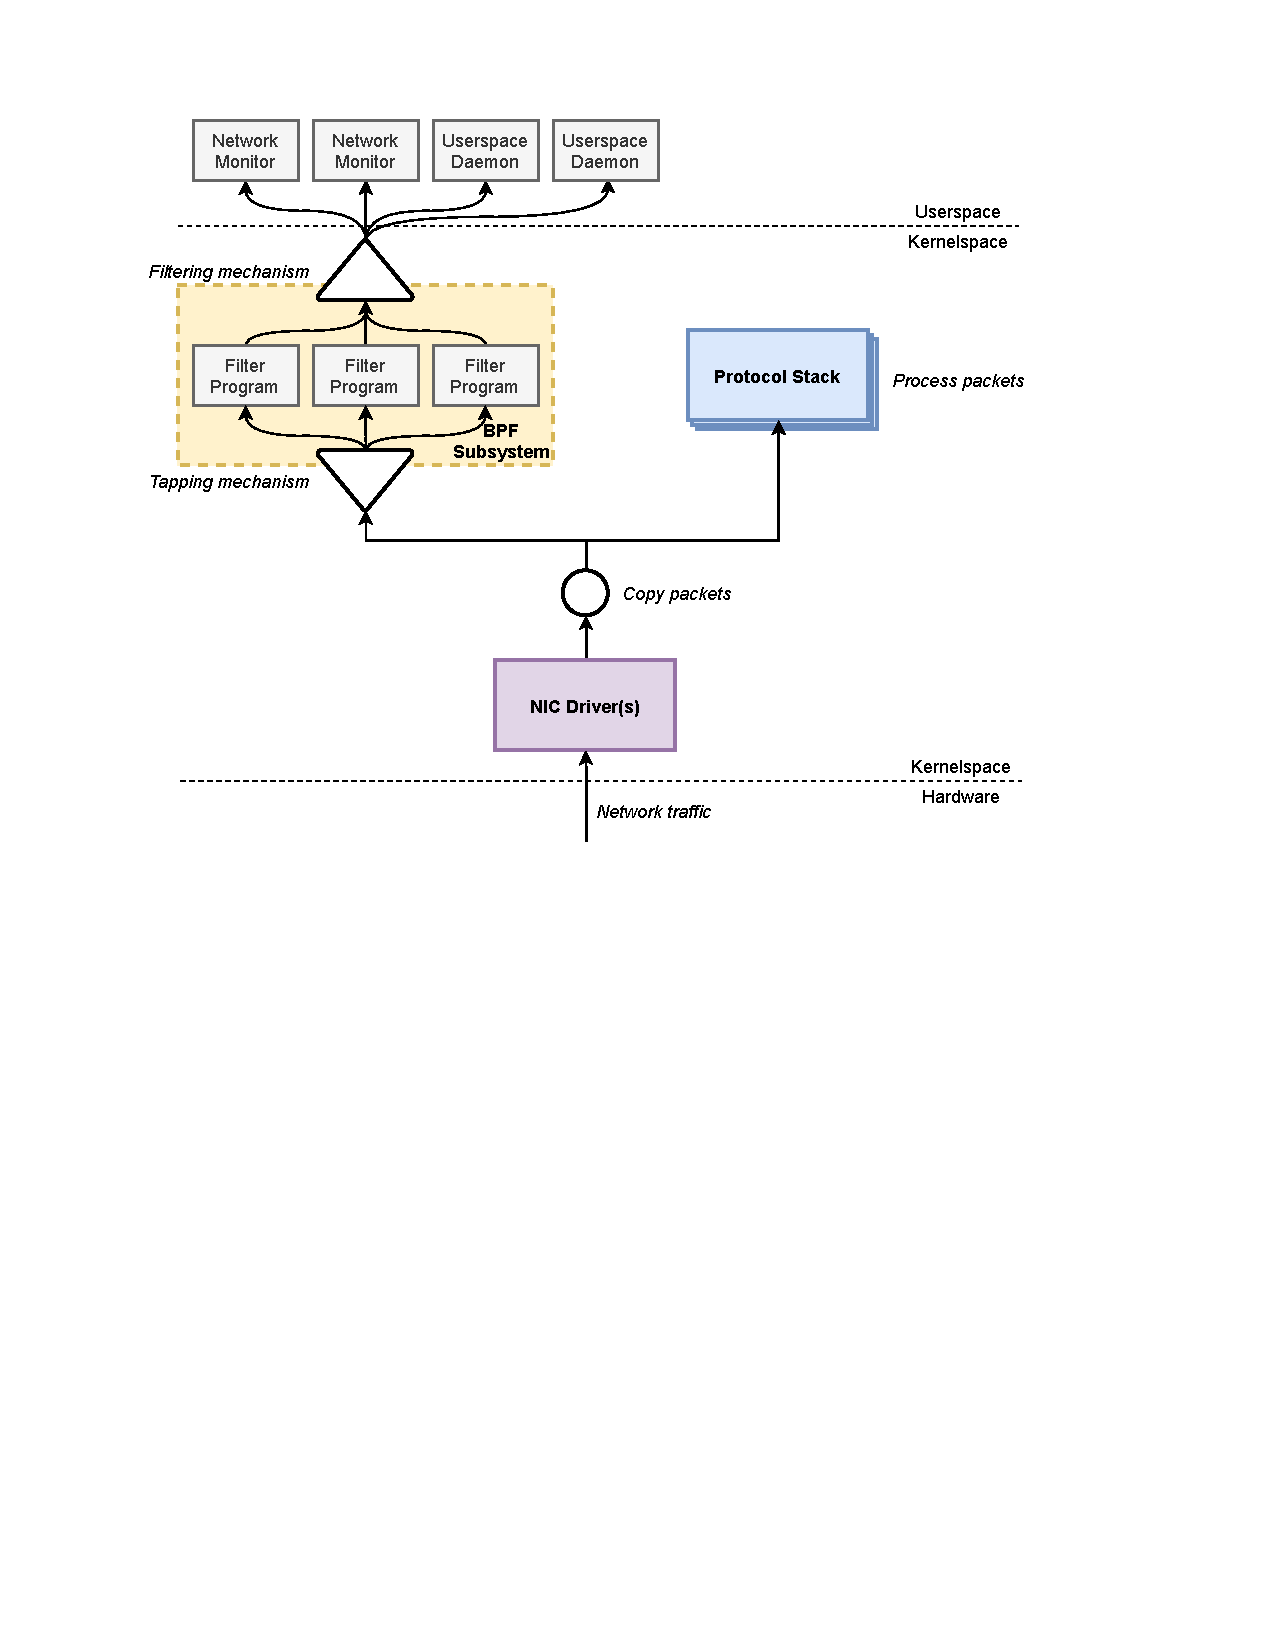
\includegraphics[width=0.8\linewidth]{figs/background/classic-bpf.pdf}
  \caption[The classic BPF architecture]{
    The classic \gls{bpf} architecture. Adapted from McCanne and Jacobson~\cite{mccanne1993_bpf}.
  }%
  \label{fig:classic-bpf}
\end{figure}

Classic \gls{bpf} can be divided into two major components: a \textit{tap} mechanism and a set
of one or more \textit{filter} programs. The cBPF architecture is depicted in
\Cref{fig:classic-bpf}. \gls{cbpf} programs are expressed as a control-flow graph (CFG)
over a set of abstract registers, backed by physical registers on the \gls{cpu}. The tap
mechanism hooks into packets as they enter the networking stack, copying and forwarding
them to the filters. At runtime, the filter programs walk their control-flow graph, taking
the forwarded packets as input. As output, they return a filtering decision which controls
whether or not the packet should be forwarded to userspace~\cite{mccanne1993_bpf}.

Since its original introduction in 1993, classic \gls{bpf} has since been ported to
a number of Unix-like operating systems, including Linux~\cite{linux_bpf},
OpenBSD~\cite{openbsd_bpf}, and FreeBSD~\cite{freebsd_bpf}. Classic \gls{bpf} forms the
backbone of widely used traffic monitoring tools, most notably tcpdump~\cite{tcpdump,
mccanne1993_bpf}. In Linux, the \texttt{seccomp(2)} system
call~\cite{anderson2017_comparison} was enhanced to include classic \gls{bpf} filters,
allowing a user process to use classic \gls{bpf} programs to define allowlists and
denylists of system calls (c.f.\ \Cref{sss:seccomp}).

In 2014, Alexei Starovoitov and Daniel Borkmann~\cite{starovoitov2014_ebpf} first proposed
a total overhaul of the Linux \gls{bpf} engine. Their proposal, dubbed \gls{ebpf}, expanded the
classic \gls{bpf} execution model into a full-fledged virtual instruction set. In particular,
the extensions included a 512 byte stack, 11 registers (10 of which are general-purpose),
the ability to call a set of allowlisted kernel helper functions, the ability to attach
programs to a variety of system events, specialized data structures (called \gls{bpf} maps) to
store and share data at runtime, and an in-kernel verification engine to check for program
safety. At runtime, programs can be dynamically attached to system events and are
just-in-time compiled into the native instruction set.  \Cref{fig:extended-bpf} depicts
the \gls{ebpf} architecture in detail. The reader is encouraged to compare this with the classic
BPF architecture, depicted in \Cref{fig:classic-bpf}.

Dtrace~\cite{cantrill2004_dtrace, gregg2001_dtrace} served as an early inspiration for the
design of \gls{ebpf} and related tooling. The original Dtrace model was to make low-level
systems tracing available to end users by exporting a simple tracing language (called D)
and supporting upstream hooking of kernel functions using this language. \gls{ebpf}
implements a superset of Dtrace's original functionality, enabling userspace applications
to hook into the kernel and other userspace applications, attaching bytecode programs to
be run as callbacks.  Userspace \gls{ebpf} tooling then simplifies the process of writing
\gls{ebpf} programs by introducing increasingly high-level layers of abstraction.

\begin{figure}[htbp]
  \centering
  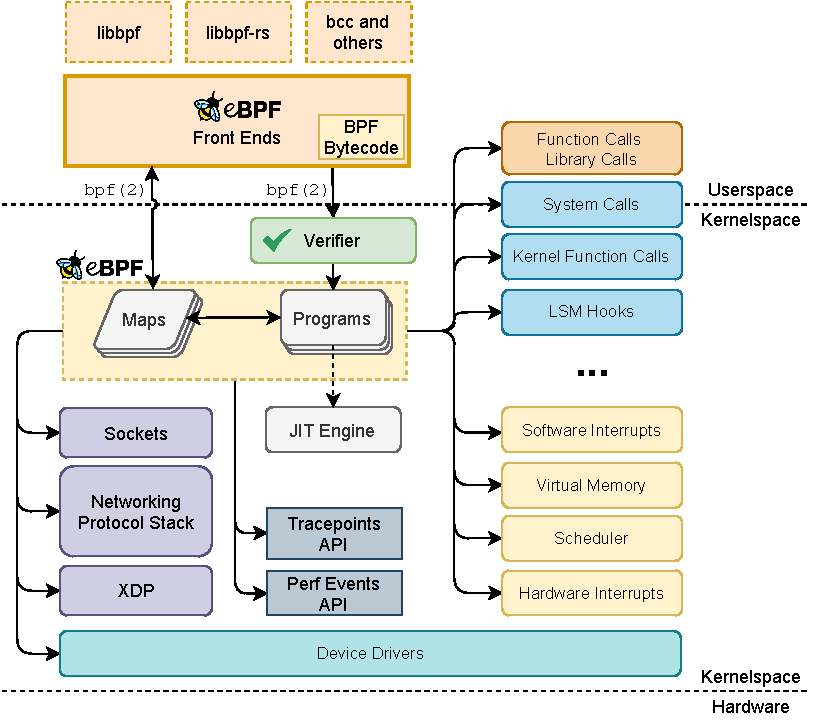
\includegraphics[width=0.8\linewidth]{figs/background/ebpf.pdf}
  \caption[The extended BPF architecture]{The extended \gls{bpf} architecture. Unlike classic
  \gls{bpf}, \gls{ebpf} programs are \gls{jit} compiled to the native instruction set, share data using
  specialized map data structures, and can be attached to many different kinds of system
  events. Programs can share data with each other and with the controlling userspace
  process using specialized map data structures. All \gls{ebpf} bytecode goes through
  a verification step before it can be loaded into the kernel.}%
  \label{fig:extended-bpf}
\end{figure}

While modern \gls{ebpf} has very little to do with the execution model of its older cousin, some
of the properties that made classic \gls{bpf} so performant still hold true today. In
particular, to notion of aggregating and processing data in kernelspace before
(optionally) handing it off to userspace is a key aspect of classic \gls{bpf} that has carried
over to \gls{ebpf}. What this means in practice is that \gls{ebpf} programs can be used to implement
very efficient monitoring software, harnessing the performance benefits of a pure
kernelspace implementation while maintaining the flexibility of a userspace
implementation.

\subsection{eBPF Programs}%
\label{ss:bpf-programs-bg}

\gls{ebpf} programs are expressed in a virtual RISC machine language called \gls{bpf}
bytecode.  While it is technically possible to write \gls{bpf} bytecode by hand, programs
are most often compiled from a restricted subset of the C programming
language\footnote{Other languages may eventually be used to write \gls{ebpf} programs as
well.  For instance, an experimental Rust \gls{ebpf} target has recently been merged into
the Rust compiler~\cite{decina2021_bpf_rust}. The important distinction here is that the
set of all possible \gls{ebpf} programs is a strict subset of the set of all possible
programs.} using the LLVM toolchain.Programs can be loaded and attached to system events
using the \texttt{bpf(2)} system call, at which point control passes to the \gls{ebpf}
verifier, which checks the programs to make sure they satisfy a set of safety
constraints~\cite{starovoitov2014_ebpf, gregg2019_bpf}.

In particular, \gls{ebpf} programs must consist of fewer than 1 million \gls{bpf}
instructions and must not call into any kernel functions outside of the allowlisted
helpers. The program is also constrained to a 512 byte stack size; any additional memory
required by the program must come from an \gls{ebpf} map (c.f.\ \Cref{ss:bpf-maps-bg}). For
safety, memory accesses into allocated buffers must be properly bounds checked, pointers
must be null-checked before dereferencing, and any access to external memory
(e.g.\ belonging to userspace programs or to the kernel itself) must be read-only. Since
\gls{ebpf} programs must provably terminate, no back-edges are permitted in their control
flow and all loops must be bounded by some fixed constant $i$ iterations.

To guard against data races, \gls{ebpf} programs always hold the kernel's RCU (read-copy-update)
lock while executing, gated by the \texttt{bpf\_prog\_enter} and \texttt{bpf\_prog\_exit}
functions in the kernel. In simple terms, the RCU lock allows concurrent reads, except in
the presence of updates, optimizing for read-mostly workloads (i.e.\ precisely the sort of
workload \gls{ebpf} is designed for)~\cite{mckenney2007_rcu}. This implicitly enables \gls{bpf}
programs to read from many common kernel data structures without fear of data races and
simultaneously protects reads and updates to \gls{ebpf} maps, at a slight (albeit reasonable)
performance penalty~\cite{mckenney2007_rcu}. In addition to holding the RCU lock, \gls{ebpf}
programs are not considered \textit{preemptable} by default. In practice, this means that
\gls{ebpf} programs cannot sleep and must run to termination on their assigned core. This
property, while useful in many circumstances, enforces undesirable limitations on \gls{ebpf}
helpers, since it precludes any functionality that may cause the program to sleep (e.g.\ a
page fault). To account for use cases where sleeping is unavoidable, Linux 5.10 introduced
sleepable versions of some \gls{ebpf} program types~\cite{starovoitov2020_sleepable}.

Once loaded into the kernel, \gls{ebpf} programs are represented as \gls{bpf} objects, each with its
own reference count. Loading a \gls{bpf} program and attaching it to a system event increments
the reference count, while detaching and unloading the program decrements the reference
count. The kernel also exposes a special filesystem, \textit{bpffs} , which allows \gls{bpf}
programs to be pinned. This also increments the reference count, allowing an attached
program to outlive its controlling process (i.e.\ the process that loaded and attached
it)~\cite{gregg2019_bpf}.

\subsubsection*{Working with the Verifier}

In practice, the restrictions imposed by the verifier mean that \gls{ebpf} programs are not
\textit{Turing-complete}~\cite{gregg2019_bpf}.  This property is required, given that the
halting problem (i.e.\ the decidability of program termination) is known not to be solvable
for Turing-complete programs. This notion of Turing-incompleteness means that the set of
all possible \gls{ebpf} programs is a strict subset of the set of all possible C programs. While
these limitations help to ensure program safety, they also naturally restrict some
operations which \textit{may} be safe but are not strictly verifiable. To overcome the
limitations imposed by the verifier and achieve this safe-yet-unverifiable behaviour, \gls{ebpf}
programmers have a few tools in their arsenal. For instance, a specific set of allowlisted
kernel helpers offers the ability to call into specific kernel functions, bypassing the
limitations imposed by the \gls{ebpf} verifier. As a simple example, the
\texttt{bpf\_probe\_write\_user()} helper allows an \gls{ebpf} program to write to a userspace
memory address, bypassing the read-only restrictions imposed by the verifier. While these
allowlisted helpers operate in a \textit{mostly} unrestricted context, their usage
\textit{is} restricted at the function call boundary, ensuring that the \gls{ebpf} program obeys
the safety contract specified by the helper function.  Another common design pattern is
using a dummy \gls{ebpf} map as a scratch buffer to reserve a larger amount of memory for the
\gls{ebpf} program.  Since \gls{ebpf} programs cannot sleep~\cite{gregg2019_bpf}, dynamic memory
allocation within the \gls{bpf} context is impossible. These dummy maps offer a way to access
additional memory from a pool reserved at the time the map was loaded into the kernel.

\subsubsection*{eBPF Program Types and Use Cases}

Each \gls{ebpf} program has a specific \textit{program type}, which determines both the
set of system events to which the program can attach and the set of allowed kernel helpers
that can be called from within the program context. Each program type roughly corresponds
with a distinct \gls{ebpf} use case. For the purposes of this thesis, we will primarily be
dealing with \textit{\gls{lsm} probes}, \textit{raw tracepoints},
\textit{uprobes/uretprobes}, \textit{kprobes/kretprobes}, \textit{fentry/fexit probes},
and \textit{\gls{usdt} probes} as they form the basis of \bpfbox{} and \bpfcontain{}'s
kernelspace implementations. \Cref{tab:program-types} summarizes the relevant program
types and their properties.

\begingroup\small
\begin{longtable}[c]{lp{4.2in}}
\caption[A selection of relevant eBPF program types for \bpfbox{} and \bpfcontain{}]{A selection of relevant \gls{ebpf} program types for \bpfbox{} and \bpfcontain{}.}%
\label{tab:program-types}\\
  \toprule
  Program Type & Description\\
  \midrule
  \textit{\gls{lsm} Probes}    & \gls{lsm} probes~\cite{singh2019_krsi} attach to the kernel's \gls{lsm} hooks and can be used to audit security events and make policy decisions.\\
  \textit{Raw Tracepoints}     & Raw tracepoint programs attach to a stable tracing interface exposed by the Linux kernel. Tracepoints are considered a stable \gls{api}, but are more limiting than alternatives such as Kprobes or Fentry probes.\\
  \textit{Kprobes/Kretprobes}  & Kprobe programs can attach to any kernel function, by replacing the function with a trap into the \gls{bpf} program. The \gls{bpf} program has read-only access to the function arguments. Kretprobes work in the same way, but handle function returns instead of function calls.\\
  \textit{Fentry/Fexit Probes} & A more efficient version of Kprobes and Kretprobes that directly trampolines into the \gls{bpf} program instead of trapping. These programs can also be used to modify the return value of specifically allowlisted kernel functions (e.g.\ system call implementations).\\
  \textit{Uprobes/Uretprobes}  & The userspace equivalent of Kprobes and Kretprobes.\\
  \textit{\glsentryshort{usdt} Probes}  & A statically defined version of uprobes and uretprobes. Application developers may place these at strategic points within an application in order to add explicit support for userspace tracing at compile-time.\\
  \bottomrule
\end{longtable}
\endgroup

\subsubsection*{LSM Probes: Making Security Decisions with eBPF}

It is worth spending more time focusing specifically on \gls{lsm} probes, as these are used
extensively in \bpfbox{} and \bpfcontain{} to enforce policy over security-sensitive
events. Introduced by KP Singh in his \gls{krsi}
patch~\cite{singh2019_krsi}, \gls{lsm} probes define a canonical framework for attaching \gls{ebpf}
programs to the Linux kernel's \gls{lsm} security hooks (c.f.\ \Cref{ss:mac}). Unlike
traditional \gls{lsm}s which are implemented as static kernel modules, \gls{lsm} probes are
\textit{dynamically attachable}, meaning that \gls{mac} and audit policy can be adjusted at
runtime, simply by loading a new \gls{ebpf} program.  \Cref{fig:bpf-lsm} depicts how \gls{lsm} probes
integrate with the \gls{lsm} framework.

\begin{figure}[htbp]
  \centering
  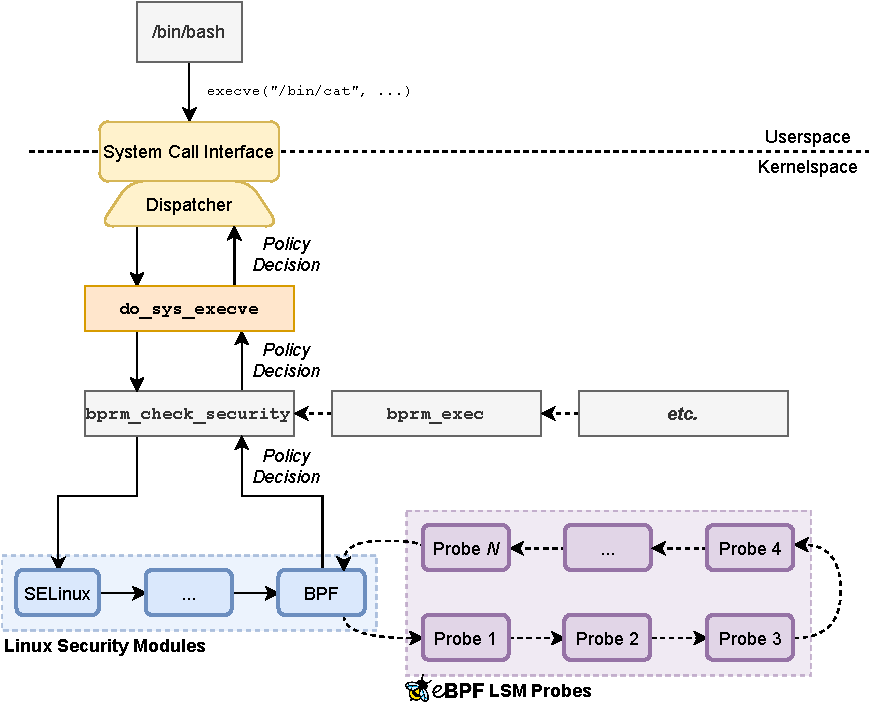
\includegraphics[width=0.8\linewidth]{figs/background/bpf-lsm.pdf}
  \caption[How eBPF LSM probes make policy decisions]{A simplified example of how \gls{ebpf} \gls{lsm} probes make policy decisions. Privileged userspace processes can attach one or more \gls{lsm} probes to a given hook. When a userspace process requests a privileged operation, the kernel implicitly calls into the corresponding \gls{lsm} hooks, which in turn invoke the logic associated with each \gls{lsm}. A shim \gls{lsm} is responsible for invoking each \gls{lsm} probe, and any resulting policy decisions are taken together to arrive at a final decision. As with ordinary \gls{lsm}s, the final decision is consensus-based. That is, if \textit{any \gls{lsm}s} or \textit{any \gls{bpf} \gls{lsm} probes} disagree on a policy decision, the privileged operation is denied.}%
  \label{fig:bpf-lsm}
\end{figure}

As with other \gls{lsm}s, \gls{lsm} probes implement a form of mandatory access control.
Each \gls{lsm} probe can be attached to one or more \gls{lsm} hooks defined in the kernel.
When the hook fires (i.e.\ when a task requests a privileged operation form the kernel),
every attached probe fires as part of the normal \gls{lsm} pipeline. The body of the
\gls{bpf} program defines filtering and audit logic, optionally accessing maps to store
and query persistent state. The \gls{bpf} program then returns a security decision about
whether the requested operation should be allowed or denied.  In order for an operation to
be allowed, \textit{all} other \gls{lsm}s and \gls{lsm} probes must agree on the policy
decision and ordinary security checks performed by the operating system must also succeed.
In other words, it is not possible to grant additional privileges using an \gls{lsm}
probe.

Owing to the properties discussed earlier in this section, \gls{ebpf} confers a natural
flexibility to \gls{lsm} probes quite unlike that of traditional \gls{lsm}-based security
frameworks.  In particular, \gls{lsm} probes can be attached at runtime and can cooperate
with other \gls{ebpf} program types using \gls{ebpf} maps (c.f.\ \Cref{ss:bpf-maps-bg}).
This notion of cooperating programs presents an opportunity to design modular policy
enforcement mechanisms that operate beyond the scope of the \gls{lsm} hooks framework
itself.  Another key advantage of \gls{lsm} probes over traditional \gls{lsm}s lies in
their adoptability.  While industry actors may be understandably reluctant to adopt
\enquote{yet another out-of-tree \gls{lsm}}, a security mechanism based on \gls{ebpf} does
not carry the same technical baggage.  \gls{ebpf} programs are safe to use in production
and can be deployed at runtime on an unmodified kernel.  This makes \gls{ebpf}
a particularly attractive target for developing new security solutions.

\subsection{eBPF Maps}%
\label{ss:bpf-maps-bg}

\gls{ebpf} maps serve as both a runtime data store for \gls{ebpf} programs and the
canonical method of communication between \gls{ebpf} programs and other \gls{ebpf}
programs, and \gls{ebpf} programs and userspace applications. Like \gls{ebpf} programs,
maps can be pinned to \textit{bpffs} to increment their reference count in the kernel.
Concurrent access to \gls{ebpf} maps from within kernelspace is protected by an implicit
RCU lock, and a spinlock concurrency primitive is exposed via a helper function to guard
map accesses between kernelspace and userspace.  From the \gls{ebpf} side, maps can be
accessed using a set of provided helper functions.  Userspace applications can access maps
using the \texttt{bpf(2)} system call or through direct memory-mapping (only available for
arrays) via \texttt{mmap(2)~\cite{gregg2019_bpf}}. While many \gls{ebpf} maps are designed
to be generic, others are highly specialized for specific use cases. \bpfcontain{} and
\bpfbox{} make use of several \gls{ebpf} map types, which are summarized in
\Cref{tab:map-types}.

\begingroup\footnotesize
\begin{longtable}[c]{lp{3.9in}}
\caption[A selection of relevant eBPF map types for \bpfbox{} and \bpfcontain{}]{A selection of relevant \gls{ebpf} map types for \bpfbox{} and \bpfcontain{}.}%
\label{tab:map-types}\\
  \toprule
  Map Type & Description\\
  \midrule
  \textit{\gls{bpf} Hashmap}           & A key-value hashmap. Keys and values can be arbitrary data structures.\\
  \textit{\gls{bpf} Array}             & A fixed-size array with integer indices. Values can be arbitrary data structures.\\
  \textit{\gls{bpf} Array/Map of Maps} & A \gls{bpf} array or map that stores handles into \textit{other maps}.\\
  \textit{\gls{bpf} Per-\glsentryshort{cpu} Array/Map} & Like a \gls{bpf} hashmap or \gls{bpf} array but with a separate copy per logical \glsentryshort{cpu}\@. This enables concurrent access across \glsentryshortpl{cpu}, but without synchronization.\\
  \textit{\gls{bpf} Local Storage}     & A dummy \gls{bpf} map that provides a handle into local storage for a given kernel data structure. For instance, task local storage provides storage per-task-struct. Values can be arbitrary data structures.\\
  \textit{\gls{bpf} Ringbuf}           & A concurrent circular buffer that passes event handles from kernelspace to userspace. To communicate, \gls{ebpf} programs submit events and userspace applications poll events.\\
  \bottomrule
\end{longtable}
\endgroup

\subsection{Userspace Front-Ends}%
\label{ss:bpf-userspace}

Although \gls{ebpf} programs and maps can exist on their own after being pinned to
\textit{bpffs}, the more common approach is to manage their lifetime using a controlling
process. Userspace applications implementing such a controlling process typically use an
\gls{ebpf} front-end framework to facilitate loading and interacting with programs and maps.
A number of such front-ends exist~\cite{gobpf, bcc, libbpf, libbpf-rs, libbpfgo,
cilium-ebpf, redbpf}, some more practical than others.
\textit{bcc}~\cite{bcc} was the first \gls{ebpf} framework to offer high-level userspace tooling
around \gls{ebpf}, providing an LLVM backend for compiling \gls{ebpf} programs and a Python library
for loading and interacting with them. \textit{libbpf}~\cite{libbpf} offers a pure
C alternative to bcc and has since been upstreamed into the Linux kernel.
\textit{libbpf-rs}~\cite{libbpf-rs} and \textit{libbpfgo}~\cite{libbpfgo} offer Rust
and Golang bindings for libbpf respectively. Other tooling~\cite{cilium-ebpf, redbpf}
bypasses libbpf entirely, providing fully native \gls{ebpf} bindings for Rust and Golang.

\subsubsection*{Libbpf and BPF CO-RE}%

Among the myriad of userspace front-ends available for \gls{ebpf}, libbpf stands out as the only
one with official upstream support from the Linux kernel. Recent improvements to libbpf
have solidified its position as the dominant framework. In particular, libbpf supports
a new way of compiling and loading \gls{bpf} programs into the kernel, \gls{bpf}
\gls{core}~\cite{gregg2020_core, nakryiko2020_core}. \gls{bpf} \gls{core} uses \gls{btf}
debugging information exposed by the kernel, along with load-time relocation logic to
support loading the same compiled \gls{ebpf} bytecode across multiple target kernels. The
precise technical details of how \gls{core} works are beyond the scope of this thesis.

With libbpf and \gls{core}, \gls{ebpf} programs can now be compiled once and run on any target kernel
that supports the required \gls{bpf} features. This provides a powerful advantage over other
\gls{ebpf} frameworks and even alternatives to \gls{ebpf}, such as loadable kernel modules. A \gls{core}
program that runs on one kernel will be guaranteed to run on another of the same version
or higher, barring any \gls{api} incompatibilities like changes in a hooker function signature.
Such incompatibilities can be resolved with the use of built-in kernel configuration
checks.

\bpfcontain{} (c.f.\ \Cref{c:bpfcontain}) leverages libbpf and \gls{core} through libbpf-rs, the
canonical Rust bindings for libbpf, providing adoptability advantages over the original
\bpfbox{} prototype (c.f.\ \Cref{c:bpfbox}), which uses bcc.

\subsection{Comparing eBPF with Loadable Kernel Modules}%
\label{ss:bpf-vs-modules}

Before \gls{ebpf}, the primary means of modifying the Linux kernel at runtime was through the
use of \textit{loadable kernel modules}~\cite{corbet1998_device_drivers}. A kernel module
can be thought of as a discrete bundle of code that can be loaded into the kernel (or
compiled into its binary image). Like other kernel code, including \gls{ebpf}, modules are
event-based and run in ring 0, responding to and handling system events as they occur.
Since kernel modules and \gls{ebpf} can serve similar (but not strictly equivalent) purposes,
comparing the two can offer some insight about how they differ and which technology is
better fit for a specific purpose.

At a first approximation, \gls{ebpf} differs from kernel modules in the following meaningful ways~\cite{gregg2019_bpf}:
\begin{enumerate}
  \item \gls{ebpf} programs \textbf{must pass verification checks} before they can be loaded into the
  kernel. This verification step provides assurances about program safety. For instance, \gls{ebpf}
  programs are guaranteed not to deadlock the kernel, and are far less likely to suffer from
  memory safety issues. In contrast, misuse of kernel \gls{api}s in a kernel module can have dangerous
  implications for system safety and security.

  \item An implicit advantage provided by \gls{ebpf} is that \gls{bpf} programs can be \textbf{easier
  to reason about} than other kernel code. \gls{ebpf} abstracts away much of the complex
  functionality required to make kernel code operate correctly by providing implicit
  guarantees about program execution. Even helper functions, which offer functionality
  beyond the scope of verifiability, must obey a predetermined contract with the verifier
  in order to be considered safe. Thus, when an \gls{ebpf} program passes verification, there is
  a much higher likelihood that it will \enquote{just work.}

  \item \gls{ebpf} \textbf{exposes map-like data structures} to facilitate runtime data storage,
  communication between \gls{ebpf} programs, and communication with userspace applications. In
  the case of kernel modules, data structures often must be implemented by hand, taking
  great care not to introduce potential bugs or security vulnerabilities, particularly in
  the case of memory management. Communication with userspace from a kernel module might
  be done via netlink sockets, file operations, or similar
  means~\cite{corbet1998_device_drivers}. These modes of communication are often less
  streamlined and, in the case of file operations, must be implemented by hand, increasing
  the likelihood of programmer error.

  \item \gls{ebpf} programs are \textbf{not Turing-complete}. Intuitively, this means that
  the set of operations a kernel module can perform is a strict superset of \gls{ebpf}. While
  this may appear to be a hugely limiting factor, in practice \gls{ebpf} programs are often
  sufficient to implement sophisticated tracing, filtering, and policy enforcement logic.
  Where the verifier gets in the way, the programmer can reach for a number of helper
  functions provided by the kernel to achieve more complex behaviour.

  \item \gls{ebpf} is \textbf{not \textit{generally} suitable for implementing device drivers} or
  other complex functionality that requires ad-hoc access to various kernel facilities and
  write access to arbitrary memory locations. Where necessary, \gls{ebpf} helpers can be
  added to the kernel to perform more complex functionality from within a \gls{bpf}
  program. However, these helpers must be upstreamed in the kernel in order to be used,
  are limited to specific program types, and must obey a safety contract with the
  verifier.
\end{enumerate}

\begin{table}[!htb]
  \centering
  \caption[A high-level comparison between \glsentryshort{ebpf}, loadable kernel
  modules, and kernel patches]{
    A high-level comparison between \glsentryshort{ebpf}, loadable kernel modules, and
    kernel patches. \fullc{} = property satisfied; \halfc{} = property somewhat satisfied;
    \emptyc{} = property not satisfied.
  }%
  \label{tab:ebpf-comparison}
  \begin{tabular}{lccccccp{4.8em}}
  \toprule
                       & \rot{45}{Loadable at Runtime} & \rot{45}{Verified Safety}
                       & \rot{45}{Easy Abstractions}   & \rot{45}{Rich Data Structures}
                       & \rot{45}{Turing Complete}     & \rot{45}{Complex Functionality} & \\
  \midrule
  \glsentryshort{ebpf} & \fullc  & \fullc  & \fullc  & \fullc  & \emptyc & \halfc  & \\
  Kernel Modules       & \halfc  & \emptyc & \emptyc & \emptyc & \fullc  & \fullc  & \\
  Kernel Patches       & \emptyc & \emptyc & \emptyc & \emptyc & \fullc  & \fullc  & \\
  \bottomrule
  \end{tabular}
\end{table}

In summary, \gls{ebpf} is useful for observability use cases, or cases in which the
functional requirements of the kernel code are not expected to be complex or might be
expected to change frequently. \gls{ebpf} programs and maps are particularly good at
separation of concerns, composability, and modularity. \gls{ebpf} maps facilitate easy
communication between kernelspace and userspace, and provide the ability to build
relationships between data from different program types. Kernel modules should be
preferred for the implementation of more complex kernel functionality, such as device
drivers. \Cref{tab:ebpf-comparison} presents a summary comparison of \gls{ebpf}, kernel
modules, and kernel patches as a means of running custom code in the kernel.
